\documentclass[11pt,a4paper,openany]{book}

%\usepackage[german]{babel}	%in case you want to write a german thesis

%settings for generation of titlepage, index and table of content
\usepackage{graphicx}
\usepackage{geometry}
\usepackage{fancyhdr}
\usepackage{tabularx}
\usepackage[style=verbose,
indexing=cite,
backend=biber,
sorting=nyt,
maxcitenames=1, 
mincitenames=1, 
maxbibnames=999, 
minbibnames=999,
refsection=section,
doi=true,
url=true]{biblatex}
\usepackage{makecell}
\usepackage{titlesec}
\usepackage{lipsum}
\usepackage[super]{nth}
\usepackage{imakeidx}
\usepackage{hyperref}
\usepackage{listings}
\usepackage{color}
\usepackage{listings}
\usepackage{tikz}
\usepackage{xcolor}
\usepackage{svg}
\usepackage{tocdata}
\usepackage{titletoc}

\definecolor{dkgreen}{rgb}{0,0.6,0}
\definecolor{gray}{rgb}{0.5,0.5,0.5}
\definecolor{mauve}{rgb}{0.58,0,0.82}
\definecolor{orange}{RGB}{255,143,0}

\lstset{frame=tb,
	language=python,
	aboveskip=5mm,
	belowskip=5mm,
	showstringspaces=false,
	columns=flexible,
	basicstyle={\small\ttfamily},
	numbers=left,
	numberstyle=\tiny\color{gray},
	keywordstyle=\color{orange},
	commentstyle=\color{dkgreen},
	stringstyle=\color{mauve},
	breaklines=true,
	breakatwhitespace=false,
	tabsize=4
}

\lstdefinelanguage{Rust}{%
  sensitive%
, morecomment=[l]{//}%
, morecomment=[s]{/*}{*/}%
, moredelim=[s][{\itshape\color[rgb]{0,0,0.75}}]{\#[}{]}%
, morestring=[b]{"}%
, alsodigit={}%
, alsoother={}%
, alsoletter={!}%
%
%
% [1] reserve keywords
% [2] traits
% [3] primitive types
% [4] type and value constructors
% [5] identifier
%
, morekeywords={break, continue, else, for, if, in, loop, match, return, while}  % control flow keywords
, morekeywords={as, const, let, move, mut, ref, static}  % in the context of variables
, morekeywords={dyn, enum, fn, impl, Self, self, struct, trait, type, union, use, where}  % in the context of declarations
, morekeywords={crate, extern, mod, pub, super}  % in the context of modularisation
, morekeywords={unsafe}  % markers
, morekeywords={abstract, alignof, become, box, do, final, macro, offsetof, override, priv, proc, pure, sizeof, typeof, unsized, virtual, yield}  % reserved identifiers
%
% grep 'pub trait [A-Za-z][A-Za-z0-9]*' -r . | sed 's/^.*pub trait \([A-Za-z][A-Za-z0-9]*\).*/\1/g' | sort -u | tr '\n' ',' | sed 's/^\(.*\),$/{\1}\n/g' | sed 's/,/, /g'
, morekeywords=[2]{Add, AddAssign, Any, AsciiExt, AsInner, AsInnerMut, AsMut, AsRawFd, AsRawHandle, AsRawSocket, AsRef, Binary, BitAnd, BitAndAssign, Bitor, BitOr, BitOrAssign, BitXor, BitXorAssign, Borrow, BorrowMut, Boxed, BoxPlace, BufRead, BuildHasher, CastInto, CharExt, Clone, CoerceUnsized, CommandExt, Copy, Debug, DecodableFloat, Default, Deref, DerefMut, DirBuilderExt, DirEntryExt, Display, Div, DivAssign, DoubleEndedIterator, DoubleEndedSearcher, Drop, EnvKey, Eq, Error, ExactSizeIterator, ExitStatusExt, Extend, FileExt, FileTypeExt, Float, Fn, FnBox, FnMut, FnOnce, Freeze, From, FromInner, FromIterator, FromRawFd, FromRawHandle, FromRawSocket, FromStr, FullOps, FusedIterator, Generator, Hash, Hasher, Index, IndexMut, InPlace, Int, Into, IntoCow, IntoInner, IntoIterator, IntoRawFd, IntoRawHandle, IntoRawSocket, IsMinusOne, IsZero, Iterator, JoinHandleExt, LargeInt, LowerExp, LowerHex, MetadataExt, Mul, MulAssign, Neg, Not, Octal, OpenOptionsExt, Ord, OsStrExt, OsStringExt, Packet, PartialEq, PartialOrd, Pattern, PermissionsExt, Place, Placer, Pointer, Product, Put, RangeArgument, RawFloat, Read, Rem, RemAssign, Seek, Shl, ShlAssign, Shr, ShrAssign, Sized, SliceConcatExt, SliceExt, SliceIndex, Stats, Step, StrExt, Sub, SubAssign, Sum, Sync, TDynBenchFn, Terminal, Termination, ToOwned, ToSocketAddrs, ToString, Try, TryFrom, TryInto, UnicodeStr, Unsize, UpperExp, UpperHex, WideInt, Write}
, morekeywords=[2]{Send}  % additional traits
%
, morekeywords=[3]{bool, char, f32, f64, i8, i16, i32, i64, isize, str, u8, u16, u32, u64, unit, usize, i128, u128}  % primitive types
%
, morekeywords=[4]{Err, false, None, Ok, Some, true}  % prelude value constructors
% grep 'pub \(type\|struct\|enum\) [A-Za-z][A-Za-z0-9]*' -r . | sed 's/^.*pub \(type\|struct\|enum\) \([A-Za-z][A-Za-z0-9]*\).*/\2/g' | sort -u | tr '\n' ',' | sed 's/^\(.*\),$/{\1}\n/g' | sed 's/,/, /g'    
, morekeywords=[3]{AccessError, Adddf3, AddI128, AddoI128, AddoU128, ADDRESS, ADDRESS64, addrinfo, ADDRINFOA, AddrParseError, Addsf3, AddU128, advice, aiocb, Alignment, AllocErr, AnonPipe, Answer, Arc, Args, ArgsInnerDebug, ArgsOs, Argument, Arguments, ArgumentV1, Ashldi3, Ashlti3, Ashrdi3, Ashrti3, AssertParamIsClone, AssertParamIsCopy, AssertParamIsEq, AssertUnwindSafe, AtomicBool, AtomicPtr, Attr, auxtype, auxv, BackPlace, BacktraceContext, Barrier, BarrierWaitResult, Bencher, BenchMode, BenchSamples, BinaryHeap, BinaryHeapPlace, blkcnt, blkcnt64, blksize, BOOL, boolean, BOOLEAN, BoolTrie, BorrowError, BorrowMutError, Bound, Box, bpf, BTreeMap, BTreeSet, Bucket, BucketState, Buf, BufReader, BufWriter, Builder, BuildHasherDefault, BY, BYTE, Bytes, CannotReallocInPlace, cc, Cell, Chain, CHAR, CharIndices, CharPredicateSearcher, Chars, CharSearcher, CharsError, CharSliceSearcher, CharTryFromError, Child, ChildPipes, ChildStderr, ChildStdin, ChildStdio, ChildStdout, Chunks, ChunksMut, ciovec, clock, clockid, Cloned, cmsgcred, cmsghdr, CodePoint, Color, ColorConfig, Command, CommandEnv, Component, Components, CONDITION, condvar, Condvar, CONSOLE, CONTEXT, Count, Cow, cpu, CRITICAL, CStr, CString, CStringArray, Cursor, Cycle, CycleIter, daddr, DebugList, DebugMap, DebugSet, DebugStruct, DebugTuple, Decimal, Decoded, DecodeUtf16, DecodeUtf16Error, DecodeUtf8, DefaultEnvKey, DefaultHasher, dev, device, Difference, Digit32, DIR, DirBuilder, dircookie, dirent, dirent64, DirEntry, Discriminant, DISPATCHER, Display, Divdf3, Divdi3, Divmoddi4, Divmodsi4, Divsf3, Divsi3, Divti3, dl, Dl, Dlmalloc, Dns, DnsAnswer, DnsQuery, dqblk, Drain, DrainFilter, Dtor, Duration, DwarfReader, DWORD, DWORDLONG, DynamicLibrary, Edge, EHAction, EHContext, Elf32, Elf64, Empty, EmptyBucket, EncodeUtf16, EncodeWide, Entry, EntryPlace, Enumerate, Env, epoll, errno, Error, ErrorKind, EscapeDebug, EscapeDefault, EscapeUnicode, event, Event, eventrwflags, eventtype, ExactChunks, ExactChunksMut, EXCEPTION, Excess, ExchangeHeapSingleton, exit, exitcode, ExitStatus, Failure, fd, fdflags, fdsflags, fdstat, ff, fflags, File, FILE, FileAttr, filedelta, FileDesc, FilePermissions, filesize, filestat, FILETIME, filetype, FileType, Filter, FilterMap, Fixdfdi, Fixdfsi, Fixdfti, Fixsfdi, Fixsfsi, Fixsfti, Fixunsdfdi, Fixunsdfsi, Fixunsdfti, Fixunssfdi, Fixunssfsi, Fixunssfti, Flag, FlatMap, Floatdidf, FLOATING, Floatsidf, Floatsisf, Floattidf, Floattisf, Floatundidf, Floatunsidf, Floatunsisf, Floatuntidf, Floatuntisf, flock, ForceResult, FormatSpec, Formatted, Formatter, Fp, FpCategory, fpos, fpos64, fpreg, fpregset, FPUControlWord, Frame, FromBytesWithNulError, FromUtf16Error, FromUtf8Error, FrontPlace, fsblkcnt, fsfilcnt, fsflags, fsid, fstore, fsword, FullBucket, FullBucketMut, FullDecoded, Fuse, GapThenFull, GeneratorState, gid, glob, glob64, GlobalDlmalloc, greg, group, GROUP, Guard, GUID, Handle, HANDLE, Handler, HashMap, HashSet, Heap, HINSTANCE, HMODULE, hostent, HRESULT, id, idtype, if, ifaddrs, IMAGEHLP, Immut, in, in6, Incoming, Infallible, Initializer, ino, ino64, inode, input, InsertResult, Inspect, Instant, int16, int32, int64, int8, integer, IntermediateBox, Internal, Intersection, intmax, IntoInnerError, IntoIter, IntoStringError, intptr, InvalidSequence, iovec, ip, IpAddr, ipc, Ipv4Addr, ipv6, Ipv6Addr, Ipv6MulticastScope, Iter, IterMut, itimerspec, itimerval, jail, JoinHandle, JoinPathsError, KDHELP64, kevent, kevent64, key, Key, Keys, KV, l4, LARGE, lastlog, launchpad, Layout, Lazy, lconv, Leaf, LeafOrInternal, Lines, LinesAny, LineWriter, linger, linkcount, LinkedList, load, locale, LocalKey, LocalKeyState, Location, lock, LockResult, loff, LONG, lookup, lookupflags, LookupHost, LPBOOL, LPBY, LPBYTE, LPCSTR, LPCVOID, LPCWSTR, LPDWORD, LPFILETIME, LPHANDLE, LPOVERLAPPED, LPPROCESS, LPPROGRESS, LPSECURITY, LPSTARTUPINFO, LPSTR, LPVOID, LPWCH, LPWIN32, LPWSADATA, LPWSAPROTOCOL, LPWSTR, Lshrdi3, Lshrti3, lwpid, M128A, mach, major, Map, mcontext, Metadata, Metric, MetricMap, mflags, minor, mmsghdr, Moddi3, mode, Modsi3, Modti3, MonitorMsg, MOUNT, mprot, mq, mqd, msflags, msghdr, msginfo, msglen, msgqnum, msqid, Muldf3, Mulodi4, Mulosi4, Muloti4, Mulsf3, Multi3, Mut, Mutex, MutexGuard, MyCollection, n16, NamePadding, NativeLibBoilerplate, nfds, nl, nlink, NodeRef, NoneError, NonNull, NonZero, nthreads, NulError, OccupiedEntry, off, off64, oflags, Once, OnceState, OpenOptions, Option, Options, OptRes, Ordering, OsStr, OsString, Output, OVERLAPPED, Owned, Packet, PanicInfo, Param, ParseBoolError, ParseCharError, ParseError, ParseFloatError, ParseIntError, ParseResult, Part, passwd, Path, PathBuf, PCONDITION, PCONSOLE, Peekable, PeekMut, Permissions, PhantomData, pid, Pipes, PlaceBack, PlaceFront, PLARGE, PoisonError, pollfd, PopResult, port, Position, Powidf2, Powisf2, Prefix, PrefixComponent, PrintFormat, proc, Process, PROCESS, processentry, protoent, PSRWLOCK, pthread, ptr, ptrdiff, PVECTORED, Queue, radvisory, RandomState, Range, RangeFrom, RangeFull, RangeInclusive, RangeMut, RangeTo, RangeToInclusive, RawBucket, RawFd, RawHandle, RawPthread, RawSocket, RawTable, RawVec, Rc, ReadDir, Receiver, recv, RecvError, RecvTimeoutError, ReentrantMutex, ReentrantMutexGuard, Ref, RefCell, RefMut, REPARSE, Repeat, Result, Rev, Reverse, riflags, rights, rlim, rlim64, rlimit, rlimit64, roflags, Root, RSplit, RSplitMut, RSplitN, RSplitNMut, RUNTIME, rusage, RwLock, RWLock, RwLockReadGuard, RwLockWriteGuard, sa, SafeHash, Scan, sched, scope, sdflags, SearchResult, SearchStep, SECURITY, SeekFrom, segment, Select, SelectionResult, sem, sembuf, send, Sender, SendError, servent, sf, Shared, shmatt, shmid, ShortReader, ShouldPanic, Shutdown, siflags, sigaction, SigAction, sigevent, sighandler, siginfo, Sign, signal, signalfd, SignalToken, sigset, sigval, Sink, SipHasher, SipHasher13, SipHasher24, size, SIZE, Skip, SkipWhile, Slice, SmallBoolTrie, sockaddr, SOCKADDR, sockcred, Socket, SOCKET, SocketAddr, SocketAddrV4, SocketAddrV6, socklen, speed, Splice, Split, SplitMut, SplitN, SplitNMut, SplitPaths, SplitWhitespace, spwd, SRWLOCK, ssize, stack, STACKFRAME64, StartResult, STARTUPINFO, stat, Stat, stat64, statfs, statfs64, StaticKey, statvfs, StatVfs, statvfs64, Stderr, StderrLock, StderrTerminal, Stdin, StdinLock, Stdio, StdioPipes, Stdout, StdoutLock, StdoutTerminal, StepBy, String, StripPrefixError, StrSearcher, subclockflags, Subdf3, SubI128, SuboI128, SuboU128, subrwflags, subscription, Subsf3, SubU128, Summary, suseconds, SYMBOL, SYMBOLIC, SymmetricDifference, SyncSender, sysinfo, System, SystemTime, SystemTimeError, Take, TakeWhile, tcb, tcflag, TcpListener, TcpStream, TempDir, TermInfo, TerminfoTerminal, termios, termios2, TestDesc, TestDescAndFn, TestEvent, TestFn, TestName, TestOpts, TestResult, Thread, threadattr, threadentry, ThreadId, tid, time, time64, timespec, TimeSpec, timestamp, timeval, timeval32, timezone, tm, tms, ToLowercase, ToUppercase, TraitObject, TryFromIntError, TryFromSliceError, TryIter, TryLockError, TryLockResult, TryRecvError, TrySendError, TypeId, U64x2, ucontext, ucred, Udivdi3, Udivmoddi4, Udivmodsi4, Udivmodti4, Udivsi3, Udivti3, UdpSocket, uid, UINT, uint16, uint32, uint64, uint8, uintmax, uintptr, ulflags, ULONG, ULONGLONG, Umoddi3, Umodsi3, Umodti3, UnicodeVersion, Union, Unique, UnixDatagram, UnixListener, UnixStream, Unpacked, UnsafeCell, UNWIND, UpgradeResult, useconds, user, userdata, USHORT, Utf16Encoder, Utf8Error, Utf8Lossy, Utf8LossyChunk, Utf8LossyChunksIter, utimbuf, utmp, utmpx, utsname, uuid, VacantEntry, Values, ValuesMut, VarError, Variables, Vars, VarsOs, Vec, VecDeque, vm, Void, WaitTimeoutResult, WaitToken, wchar, WCHAR, Weak, whence, WIN32, WinConsole, Windows, WindowsEnvKey, winsize, WORD, Wrapping, wrlen, WSADATA, WSAPROTOCOL, WSAPROTOCOLCHAIN, Wtf8, Wtf8Buf, Wtf8CodePoints, xsw, xucred, Zip, zx}
%
, morekeywords=[5]{assert!, assert_eq!, assert_ne!, cfg!, column!, compile_error!, concat!, concat_idents!, debug_assert!, debug_assert_eq!, debug_assert_ne!, env!, eprint!, eprintln!, file!, format!, format_args!, include!, include_bytes!, include_str!, line!, module_path!, option_env!, panic!, print!, println!, select!, stringify!, thread_local!, try!, unimplemented!, unreachable!, vec!, write!, writeln!}  % prelude macros
}%

\lstdefinestyle{colouredRust}%
{ basicstyle=\ttfamily%
, identifierstyle=%
, commentstyle=\color[gray]{0.4}%
, stringstyle=\color[rgb]{0, 0, 0.5}%
, keywordstyle=\bfseries% reserved keywords
, keywordstyle=[2]\color[rgb]{0.75, 0, 0}% traits
, keywordstyle=[3]\color[rgb]{0, 0.5, 0}% primitive types
, keywordstyle=[4]\color[rgb]{0, 0.5, 0}% type and value constructors
, keywordstyle=[5]\color[rgb]{0, 0, 0.75}% macros
, columns=spaceflexible%
, keepspaces=true%
, showspaces=false%
, showtabs=false%
, showstringspaces=true%
}%

\lstdefinestyle{boxed}{
  style=colouredRust%
, numbers=left%
, firstnumber=auto%
, numberblanklines=true%
, frame=trbL%
, numberstyle=\tiny%
, frame=leftline%
, numbersep=7pt%
, framesep=5pt%
, framerule=10pt%
, xleftmargin=15pt%
, backgroundcolor=\color[gray]{0.97}%
, rulecolor=\color[gray]{0.90}%
}

\lstdefinelanguage{ProtoBuf}{
	morestring=[b]{"},
	morekeywords=[1]{package, syntax, message, enum, oneof, option, service, returns},
	morekeywords=[2]{string, rpc, field\_type, bytes},
	stringstyle=\color[rgb]{0, 0, 0.5},
	keywordstyle=[1]\color[rgb]{0.0, 0.5, 1.0}, %Azure
	keywordstyle=[2]\color[rgb]{0.0, 0.6, 0.0}, %Dark green
	columns=spaceflexible
}

%\lstdefinelanguage{CMake}{
%	morecomment=[l]{#},
%	morestring=[b]{"},
%	morekeywords=[1]{cmake\_minimum\_required, project, set, file, find\_package, add\_library, target\_link\_libraries, target\_include\_directories, get\_target\_property, target\_compile\_definitions},
%	morekeywords=[2]{CMAKE\_CURRENT\_BINARY\_DIR},
%	commentstyle=\color[gray]{0.4},
%	stringstyle=\color[rgb]{0, 0, 0.5},
%	keywordstyle=[1]\color[rgb]{0.0, 0.5, 1.0}, %Azure
%	keywordstyle=[2]\color[rgb]{0.0, 0.5, 1.0} %Azure
%}



\lstdefinelanguage{Doxygen}{
	morecomment=[l]{//},
	morecomment=[l]{///},
	morecomment=[l]{//!},
	morecomment=[s]{/**}{*/},
	morecomment=[s]{/*!}{*/},
	morekeywords=[1]{fn, param, brief},
	commentstyle=\color[rgb]{0.0, 0.6, 0.0},
	keywordstyle=[1]\color[rgb]{0.0, 0.5, 1.0}, %Azure
	columns=spaceflexible
}

\pagestyle{fancy}
\fancyhf{}
\setlength{\headheight}{45pt}

\lhead{
  
\includegraphics[width=3cm]{img/htlwrn_logo}  
}
\chead{\Large HTBLuVA Wiener Neustadt \\ \normalsize Höhere Lehranstalt für Informatik}
\rhead{
  
\includegraphics[width=3cm]{img/htlwrn_logo2}
}

\newcommand{\parseauthor}[3]{\makecell{#1 \\ #2} & & #3}

\def \title {\Huge \bf D\,I\,P\,L\,O\,M\,A\,R\,B\,E\,I\,T}

\setlength{\parindent}{0em}

\geometry{
 a4paper,
 left=30mm,
 top=50mm,
 }
 
\graphicspath{ {img/} }

\makeindex[title=Index]
\makeindex[name=allgemein, title=Common Index]
\makeindex[name=name,title={Authors Index}]
	% do not even think about changing this from name to author
\makeindex[name=title,columns=1,title={Literature Index}]
\indexsetup{level=\subsection*, toclevel=subsection, noclearpage}


\makeatletter
\@ifpackageloaded{biblatex_legacy}
{\DeclareIndexNameFormat{default}{%
		\usebibmacro{index:name}{\index[name]}{#1}{#3}{#5}{#7}}}
{\DeclareIndexNameFormat{default}{%
		\usebibmacro{index:name}{\index[name]}
		{\namepartfamily}
		{\namepartgiven}
		{\namepartprefix}
		{\namepartsuffix}}}
\makeatother

\DeclareIndexFieldFormat{indextitle}{%
	\usebibmacro{index:title}{\index[title]}{#1}}

\renewbibmacro*{bibindex}{%
	\ifbibindex
	{\indexnames{author}%
		\indexnames{editor}%
		\indexnames{translator}%
		\indexnames{commentator}%
		\indexfield{indextitle}}
	{}}

\makeatletter
\DeclareCiteCommand{\repeatfootcite}[\cbx@wrap]
{\gdef\cbx@keys{}}
{\xappto\cbx@keys{\thefield{entrykey},}}
{}
{\ifcsundef{cbx@lastin@\cbx@keys @\strfield{postnote}}
	{\csnumgdef{cbx@lastin@\cbx@keys @\strfield{postnote}}{-1}}{}%
	\ifsamepage{\value{instcount}}{\csuse{cbx@lastin@\cbx@keys @\strfield{postnote}}}
	{\footnotemark[\csuse{cbx@lastfn@\cbx@keys @\strfield{postnote}}]}
	{\xappto\cbx@cite{\noexpand\footcite%
			[\thefield{prenote}][\thefield{postnote}]{\cbx@keys}%
			\csnumgdef{cbx@lastfn@\cbx@keys @\strfield{postnote}}{\value{\@mpfn}}%
			\csnumgdef{cbx@lastin@\cbx@keys @\strfield{postnote}}{\value{instcount}}}}}

\newrobustcmd{\cbx@wrap}[1]{#1\cbx@cite\gdef\cbx@cite{}}
\def\cbx@cite{}
\makeatother

%Messbox zur Druckkontrolle:
\newcommand{\Messbox}[2]{% Parameters: #1=Breite, #2=Hoehe
	\setlength{\unitlength}{1.0mm}%
	\begin{picture}(#1,#2)%
	\linethickness{0.05mm}%
	\put(0,0){\dashbox{0.2}(#1,#2)%
		{\parbox{#1mm}{%
				\centering\footnotesize 
				%{\bf MESSBOX}\\ 
				Breite $ = #1 {\rm\ mm}$\\
				H\"ohe $ = #2 {\rm\ mm}$
	}}}\end{picture}
}


%definitions for easier costumization
\def \subtitle {Robot Extensible Communication Toolkit}
\def \year {2023/24}
\def \authors { \parseauthor{Projectmanagement. Rust TCP/UDP and BLE Interface}{Jeremy Sztavinovszki}{5CHIF}\\
	\parseauthor{Rust gRPC Interface and interacting with in memory sqlite databases}{Christoph Fellner}{5BHIF} \\
	\parseauthor{C++ gRPC interface and library for communication}{Maximilian Dragosits}{5CHIF} \\
	\parseauthor{RECT Tool and Python gRPC interface and library for communication}{Timon Koch}{5CHIF} }
\def \supervisor { Harald R. Haberstroh }
\def \declauthors{ 	Jeremy Sztavinovszki & Christoph Fellner \\
	Timon Koch & Maximilian Dragosits}
% \def \declauthors{ Vor- und NACHNAME & Vor- und NACHNAME \\ Vor- und NACHNAME}	% for three authors

\addbibresource{main.bib}

\begin{document}
	%include titlepage
	\begin{titlepage}
  \thispagestyle{fancy}
  \begin{center}
    \Huge
    \texttt{\textbf{\title}} \\
    \vspace{1cm}
    \LARGE
    \bf{\subtitle}\\
  \end{center}
  \vspace{2cm}
  \begin{flushleft}
    \normalsize
    \textbf{Ausgeführt im Schuljahr \year \ von:}\\
    \vspace{2mm}
     \begin{tabularx}{\linewidth}{lXr}
        \authors
      \end{tabularx} \\
  \end{flushleft}
  \vfill
  \begin{center}
      \vspace{1cm}
      \textbf{Betreuer / Betreuerin:}\\
    \vspace{2mm}
    \begin{tabular}{l}
      \supervisor
    \end{tabular}
    
    \vspace{2cm}
    
    Wiener Neustadt, am \today
    
    \rule{14cm}{0.4mm}
    
    \begin{tabular}{p{.4\textwidth}p{.4\textwidth}}
      \scriptsize{Abgabevermerk:} & \scriptsize{Übernommen von:}
    \end{tabular}
    
  \end{center}
\end{titlepage}

	
	%include acknowledgements, abstract and documentation
	
	\pagestyle{plain}
	
	\frontmatter
	
	\pagenumbering{roman}
	% english word for 'eidestattliche erklärung?'

\chapter{Eidestattliche Erklärung}

\vspace{10mm}

\normalsize
Hiermit erkläre ich an Eides statt, dass ich die vorliegende Arbeit selbstständig und ohne fremde Hilfe verfasst und keine anderen als die im Literaturverzeichnis angegeben Quellen und Hilfsmittel verwendet habe. Insbesondere versichere ich, dass ich alle wörtlichen und sinngemäßen Übernahmen aus anderen Werken als solche kenntlich gemacht habe.

\vspace{1cm}

Wiener Neustadt am \today \\

\vspace{1cm}

{\bf Verfasser / Verfasserinnen:} \\

\renewcommand{\arraystretch}{5}
  \begin{tabular}{p{.4\textwidth}p{.4\textwidth}}
    \declauthors
  \end{tabular}
\renewcommand{\arraystretch}{1}
	
	\tableofcontents
	
	\chapter{Acknowledgement}

The authors would like to thank their respective families, the HTBLuVA and robo4you 
for their support throughout the process of creating this diploma thesis. 

	\chapter{Kurzfassung}

\textbf{Author: Sztavinovszki}

\vspace{10mm}

Eine der am meisten in der Robotik verwendeten Software Suiten ist das sogenannte Robot Operating System \footcite{ros-site} (kurz ROS).
Es ist eine Sammlung von Werkzeugen und Packeten, die verwendet werden, um hoch performante Robotik Systeme zu entwickeln und es abstrahiert
die Kommunikation zu Topics und Messages, die man in ROS-Bag Files aufzeichnen und abspielen kann. Das erlaubt es entwicklern sich auf die tatsächlichen Probleme der Entwicklung zu konzentrieren und sich nicht darum kümmern zu müssen Kommunikation neu zu implementieren.
ROS erlaubt außerdem die simulation Zahlreicher Komponenten von Robotern, welche man meistens als Digitale Zwillinge bezeichnet.
Einer der größten Nachteile, die ROS mit sich bringt ist die Komplexität und der Eigensinn, bei der Entwicklung. Diese Komplexität führt außerdem zu Performance einbußen, welche vor allem die Verwendbarkeit auf weniger Leistungsstarken Geräten, wie zum Beispiel dem KIPR Wombat Controller \footcite{wombat-controller}, welcher bei Schülern wegen seiner Kostengünstigkeit und Verwendbarkeit zum Einsatz kommt.

\medskip

Diese Arbeit wird erkunden, wie man eine Software ähnlich zu ROS implementiert. Es werden Probleme, wie zum Beispiel Inter Prozess Kommunikation \footcite{ipc-begriff}, Kommunikation durch Bluetooth Low Energy (BLE), TCP und UDP, und die Implementation von Kommunikations Libraries für verschiedene Programmiersprachen


\chapter{Abstract}

\textbf{Author: Sztavinovszki}

\vspace{10mm}


% Context or background information; general topic; specific topic.
In robotics one of the most important topics over the last couple of years has been communication. Communication doesn't only concern a robot being remote controllable. Mimimi keine Ahnung. 

% central questions or problem statement

% what's already known, what previous research has shown

% main reasons, rationale, goal for research

% research and or analytical methods

% main findings, results or arguments

% significance or implications


	
	%include thesis
	
	\mainmatter
	\pagenumbering{arabic}
	
	\chapter{Introduction}


\vspace{2mm}

\section{Motivation}
\textbf{Author: Sztavinovszki}
In almost every robotics application nowadays you need some kind of communication. Wether it is a robot communicating
its data to a home-base, or two robots sharing data with one another. Over the past years communication has drastically
improved with new protocols and technology, such as Bluetooth Low energy.

\section{Goal}
\textbf{Author: Sztavinovszki}

\section{History}
\textbf{Author: Dragosits}
The history of communication and coordination between seperate systems is long and extensive. Nowadays it is an essential 
function of almost every technological device. In the field of computing it started in the late 1950s with SAGE (Semi-Automatic Ground Enviornment),
which was a network of computers and networking technology created by the United States of America military, 
and it allowed the transfer of radar data nation-wide.\footcite[][89]{A_New_History_of_Modern_Computing}
The next major step forward was the beginning of ARPANET in 1969, which served as a connection between multiple north american 
universities, and laid the groundwork for the modern internet.\footcite[][25]{How_the_web_was_born}
In more recent times is the internet of things commonplace, and is used for the interchange of terabytes of data each day.

\section{Project Management}
\textbf{Author: Sztavinovszki}

\section{Outline}
%\section{Section}
%More text. \lipsum[1] See Figure~\ref{pic:example}.

%\begin{figure}[h]
%	\centering
%	\includegraphics[width=2.5in]{img/example.png}
%	\caption{Picture description.}
%	\label{pic:example}
%\end{figure}

%\subsection{Subsection}
%\lipsum[1]

%\subsection{Subsection}
%\lipsum[1] See Table~\ref{tab:example}.

%\begin{center}
%	\begin{tabular}{| l | l | l |}
%		\hline
%		\bfseries Header 1 & \bfseries Header 2 & \bfseries Header 2 \\
%		\hline
%		Text & text & text \\
%		\hline
%		Text & text & text  \\
%		\hline
%		Text & text & text  \\
%		\hline
%	\end{tabular}
%	\label{tab:example}
%\end{center}

%\lipsum[1] Some references can be found at \footcite{robo4you} or at \footcite{Hope_Learning_TensorFlow}.
%

\filbreak

	%\tocdata{toc}{$\rightarrow$\textit{Jeremy Sztavinovszki}}
\chapter{Study of Literature Sztavinovszki}

\textbf{Author: Jeremy Sztavinovszki} 

\section{The Rust Book}
% summary and main takeaway


\section{Network Programming with Rust}
% summary and main takeaway



\section{Main Takeaways}

\section{Getting Started with Bluetooth Low Energy}
Getting Started with Bluetooth Low Energy\footcite{ble_book} is a book giving deep insight into
the inner workings of Bluetooth Low Energy. The first four chapters are especially useful to this
work and are summed up in the following sections.

\subsection{Chapter 1. Introduction}
The introduction explains the history of Bluetooth Low
Energy from its start as Wibree, over the adoption by the Bluetooth Special Interest Group, to
the status at the time of the writing of the book. The chapter then goes on to explain the difference
to Bluetooth Classic. Key Limitations like Data througput and Operation range as well as possible network
topologies and the difference of Protocols versus profiles are also explained.  

\subsection{Chapter 2. Protocol Basics}
The second chapter goes over the different layers and protocols of Bluetooth Low Energy explaining the importance
and use for each of the layers and also covering the Generic Attribute Profile and the Generic Access Profile. It
provides explanations for the frequency hopping and modulation done in the physical layer and many other specifics
in the other layers.

\subsection{Chapter 3. GAP(Advertising and Connections)}
The third chapter explains concepts like roles, such as Broadcaster and Observer, and explains how each of them work.
It gives explanations of the modules and procedures included in the General Access Profile. After that section the Security
Manager and General Security constructs, such as Address Types, Authentication and Security Modes are covered. Lastly the GAP
service and the format in which data is sent over advertisements is covered.

\subsection{Chapter 4. GATT(Services and Characteristics)}
This chapter goes on to explain the roles defined in the Generall Attribute Profile and covers UUIDs.
Then the most important concept, Attributes, are explained. This chapter along with the documentation for the library this work uses for BLE solidified, that L2CAP is more suitable for this work. 
% Bla bla bla. Hier weiter schreiben.

\subsection{The Remaining Chapters}
The remaining covers go over specific hardware platforms, debugging tools, application design tools and platform specific mobile
programming and were not as important as the previous four chapters. Therefore they are not covered here.

\subsection{Main Takeaways}
The book provides great explanations of many difficult topics through text as well as visual aids. The main takeaways for this work are, that L2CAP is better suited for its purposes and better general knowledge of the BLE and its stack.


\filbreak

	%\chapter{Methodology}

\textbf{Author: } 

\filbreak

	\chapter{Methods}

\tocdata{toc}{$\rightarrow$\textit{Timon Koch}}
\section{Wombat}
\textbf{Author: Timon Koch}
The KIPR Wombat is the Controller currently used in the Botball competition. It consists of a raspberry pi 3b, a display and a casing, designed to include all necessery elements needed for the competition, such as ports for the various sensors, motors and servos allowed to be used and a cutout for the battery needed to power the used parts. Through the use of a raspberry pi 3b it is capable of wireless LAN and Bluetooth Low Energy. The Wombat uses the KISS (KIPR Instructional Software System) Web IDE developed by the KISS Institute for Practical Robotics. The current version supports ANSI C and can be used with a web browser and WiFi on any operating system.

\tocdata{toc}{$\rightarrow$\textit{Timon Koch}}
\section{Python}
\textbf{Author: Timon Koch}
Python is a powerful high-level, general purpose, object-oriented progrmming language with a design philosophy that emphasizes the readability of the written code through the use of significant indentation. 
It was created by Dutch programmer Guido van Rossum as a successor to ABC and was first released in 1991 with the capability of exepction handling. 
Features such as list comprehensions, reference counting, Unicode support and cycle-detecting garbage collections were introduced with Python 2.0 on 16 October 2000. After this release Python became a community-driven, open source project.
Due to a lack of backward compability, the switch from 2.7 to the 3.0 update, released in 2008, caused a big controversy. Folowing this most programs written in 2.7 had to be rewritten to support 3.0 update. 
Python has gained enormous popularity since the first release in the early 1990s and is used in a wide range of applications, ranging from web development to machine learning. 
The most important feature of the programming language Python is its support for mulitple programming paradigms, including object-oriented, imperative and functional programming. It was designed to be highly extensible via modules, rather than building all of itfunctionality into its core.

\tocdata{toc}{$\rightarrow$\textit{Maximilian Dragosits}}
\section{C++}
\textbf{Author: Maximilian Dragosits}

C++ is a precompiled programming language that combines low-level memory management with support for object-oriented, generic, and functional programming paradigms. 
It was designed by Danish computer scientist Bjarne Stroustrup with a focus on efficiency, performance, and flexibility.\footcite{lecture_essence_cpp} C++ has 
become widely used in various domains, including desktop applications, servers, video games, and digital equipment for space exploration.\\

It was standardized by the International Organization for Standardization (ISO) in 1998 as ISO/IEC 14882:1998 and has since evolved into a powerful programming 
language. The popularity of C++ has led to the creation of numerous libraries and frameworks, such as Catch2\footcite{catch2_git} and Doxygen\footcite{doxygen_main_site}. 
These frameworks are essential to the project's development and functionality.\\

C++ was chosen as one of the two frontend languages for this project due to its impressive speed and efficiency, as well as the vast ecosystem of external 
frameworks and libraries already available. The resources are essential in developing the RECT library, improving the project's capabilities and accelerating 
the development process. The decision to use C++ was a strategic choice, aligning with the language's strengths and the abundance of tools and resources it 
offers to the development landscape.

\tocdata{toc}{$\rightarrow$\textit{Jeremy Sztavinovszki}}
\section{Rust}
\textbf{Author: Jeremy Sztavinovszki}

Rust is a general purpose multi paradigm programming language used in many fields ranging from embedded programming to web development. Although it is a relatively young language, having released its version 1.0 on May 15th 2015, it has seen great adoption from developers and has a big community. The language tries to be as fast as possibly, while still remaining memory-safe, which it achieves using its borrow checker. Even though it is possible to write unsafe code in Rust, that is not checked by the borrow checker, it is custom to keep the unsafe parts as small as possible.
Rust has a great ecosystem driven by the Rust Foundation and the Rust community. There are many tools, such as cargo, or rust-gdb, that provide great developer experience.
Right now there is now standardized async-runtime, so you normally use runtimes like tokio, async-std, or smol for programming asynchronously.

\subsection{Documentation}
In order to provide an easy understanding of a Rust crate and its functionalities, a documentation is needed.
Documentation in Rust works by using comments in the code, which are then parsed by the \verb+cargo doc+ command. 
This command generates a folder called \verb+target/doc+ in the project, which contains the documentation in HTML format.
Comments which go into the documentation are written in a specific way.
The following is an example of this: 

\begin{minipage}{\textwidth}
  \begin{lstlisting}[language=Rust, caption=Example of a Documentation Comment]
    //! This is a module/crate-level documentation comment.

    /// This function does something
    /// # Arguments
    /// * `x` - The first parameter
    /// * `y` - The second parameter
    /// # Returns
    /// The sum of `x` and `y`
    fn add(x: i32, y: i32) -> i32 {
      x + y
    }
  \end{lstlisting}
\end{minipage}

As shown in the example, there are crate-, or module-level and general documentation comments. 
The crate-level comments are used to describe a whole crate, or module and provide an overview of the functionality of the crate or module.
The general comments are used to describe functions, structs, enums, traits, etc. and provide 
an explanation of the functionality of the specific item. The documentation for the CommLib can be found in % keine ahnung. appendix a

\tocdata{toc}{$\rightarrow$\textit{Christoph Fellner}}
\subsection{Cargo}
\textbf{Author: Christoph Fellner}

Cargo\footcite{cargo} is a build system and package manager for Rust, providing developers with a robust toolset for managing Rust projects. A rust package consists of a
\verb+Cargo.toml+ file, which contains metadata about the package, and a \verb+src+ folder, which contains the source code as rust-files (\verb+.rs+). It is an integral 
part of the Rust ecosystem and plays a crucial role in managing dependencies, building projects, and facilitating a smooth development workflow.

Here's an overview of Cargo's main functionalities:

\begin{itemize}
    \item 1. Dependency Management: Cargo manages project dependencies by automatically fetching and incorporating external libraries or crates. Developers specify 
        dependencies in the Cargo.toml file, and Cargo ensures the correct versions are used.
    \item 2. Project Structure: Cargo establishes conventions for organizing Rust projects, defining a standardized layout for directories and files. This consistency 
        helps developers understand and contribute to projects more easily.
    \item 3. Building and Compilation: Cargo handles the complexities of building and compiling Rust projects. Developers can use simple commands such as \verb+'cargo build'+ to 
        compile the code and \verb+'cargo run'+ to execute the compiled binary.
    \item 4. Testing: Cargo supports the integration of unit tests into Rust projects. Developers can use the \verb+'cargo test'+ command to run test suites, ensuring the 
        reliability and correctness of their code.
    \item 5. Documentation Generation: Cargo can generate documentation for Rust projects, making it easier for developers to create and maintain documentation for their 
        code. The \verb+'cargo doc'+ command generates and hosts documentation, and it can be published on platforms like \verb+docs.rs+.
    \item 6. Project Initialization: Cargo provides a convenient way to initialize new Rust projects with the \verb+'cargo new'+ command. This command sets up a new project with 
        the necessary directory structure and initial files.
    \item 7. Publishing: Cargo facilitates the process of publishing Rust packages (crates) to the official package registry, crates.io. This makes it straightforward for 
        developers to share their libraries and projects with the wider Rust community.
\end{itemize}

In essence, Cargo streamlines various aspects of Rust development, offering a standardized and efficient workflow for managing dependencies, building projects, testing 
code, generating documentation, and publishing packages. Its integration with the Rust toolchain contributes to the language's reputation for being developer-friendly and 
conducive to building robust and reliable systems.

\tocdata{toc}{$\rightarrow$\textit{Maximilian Dragosits}}
\section{gRPC}
\textbf{Author: Maximilian Dragosits}

gRPC\footcite{grpc_main_site} is an open-source framework that facilitates Remote Procedure Calls (RPC) across diverse environments. It is versatile 
and can be used in a broad spectrum of use cases, proving invaluable in establishing robust service-to-service connections. gRPC plays a pivotal role in the 
development of microservices and libraries. This framework is available in 11 different programming languages and provides developers with a flexible 
and accessible toolset for creating efficient and scalable communication channels.\\

gRPC's efficiency is central to its straightforward service definition and generation structure, which streamlines the integration process. 
This simplicity allows developers to focus on the core aspects of their projects, enhancing productivity and code maintainability. Furthermore, gRPC includes 
pluggable features such as authentication, load balancing, tracing, and health checking. These features provide developers with fine-grained control over 
service communication, ensuring robust and secure interactions within distributed systems.\\

In the context of the current project, gRPC plays a pivotal role. Its capability to seamlessly connect clients to backend services is particularly crucial. 
This feature enables efficient communication between Python and C++ frontends and the Rust backend, creating a cohesive and interoperable system. The project 
uses gRPC to achieve high communication efficiency, allowing for seamless data exchange between components and improving the overall performance and reliability 
of the system architecture.

\tocdata{toc}{$\rightarrow$\textit{Maximilian Dragosits}}
\section{Protocol Buffers}
\textbf{Author: Maximilian Dragosits}

Protocol Buffers offer a platform-neutral solution for serializing structured data, similar to formats such as XML, JSON, or YAML. They provide a versatile 
solution that seamlessly interfaces with automatically generated source code across an array of programming languages, catering to developers' preferences. 
Noteworthy among the supported languages are Java, Kotlin, Python, and various C-based languages, underscoring the broad applicability of Protocol Buffers 
in diverse development ecosystems.\\

Protocol Buffers enable developers to efficiently manage and exchange structured data across different platforms and systems. They provide a unified approach 
to serialization, whether using the robustness of Java, the conciseness of Kotlin, the flexibility of Python, or the performance advantages of C-based languages. 
This approach promotes interoperability, enabling developers to easily incorporate serialized data into their projects, thereby enhancing the efficiency and 
maintainability of their codebases.\\

An example of a Protocol Buffer file illustrates the elegance and conciseness inherent in this technology, demonstrating its role in facilitating efficient 
data interchange.

\begin{minipage}{\textwidth}
\begin{lstlisting}[language=ProtoBuf]
    syntax = "proto3";
    package msg;
    
    
    message From {
      string conn_name = 1;
      string topic = 2;
    }
    
    
    message To {
      string conn_name = 1;
      string topic = 2;
    }
    
    
    message Msg {
      bytes data = 1;
      oneof fromto {
        From f = 2;
        To t = 3;
      }
    }
\end{lstlisting}
\end{minipage}

As can be seen in this example the first part of any .proto file is the definition of the protobuf language version. Either \textit{proto2} or \textit{proto3}. Next the package within this will be 
stored in when it is converted into a programming languages code is defined. In this case it will be \textit{msg}. After that you can import any other .proto file.
Then it is possible to define any amount of the following types and many others not used by this project:
\begin{enumerate}
    \item \textbf{message:} Defines a special data structure that houses multiple variables of potentialy different data types, which can then be used in other enums or services.
    \item \textbf{enum:} Defines an enum which acts like the equivalent type of structure in other programming languages. This can then be used in other parts of then .proto file.
    \item \textbf{service:} Defines a Remot Procedure Call (RPC) system. The generated code for this will include service interfaces and stubs to be used by RPC frameworks.
\end{enumerate}

\subsection{Protofile message definition}

Message types in proto3 are relatively simple to define.

\begin{minipage}{\textwidth}
\begin{lstlisting}[language=ProtoBuf]
    message message_name {
        field_type field_name = number;
      }
\end{lstlisting}
\end{minipage}

First the \textit{message} keyword is used to signify that the following is a declaration for a message type. Then a freely choose able \textit{message\_name} is 
used as the name for the later resulting message structure. After that any number of fields can be defined within the curly brackets. The \textit{field\_type} can be
one of multiple supported data types, which includes but is not limited to double, flout, integer, boolean, string as well as bytes. After defining an appropriate
\textit{field\_name} this format requires the assignment of a number between 1 and 536,870,911 to each field in a message. This is required in order to identify
the field after encoding.

There are also three other modifiers, that can be applied to fields:

\begin{enumerate}
    \item \textbf{optional:} If a field with this modifier does not have its value explicitly set later it will instead return a default value. It also possible to check if this it has been set.
    \item \textbf{repeated:} A field with this modifier can be repeated any number of times within the message and the order of the repetition will be saved.
    \item \textbf{map:} A field with this modifier acts like a key/value pair with the definition syntax being like that of a C++ map.
\end{enumerate}

Another way of defining fields, that can have a multitude or a currently unkown type, is to use either the \textit{any} or the \textit{oneof} types.
The \textit{any} type is then later resolved by Protobufs internal reflection code.
\textit{Oneof} is then automatically later defined as one of the given data types within curly brackets placed after the \textit{field\_name} is given.

\subsection{Protofile enum definition}

Enums are share a lot of the same traits as message types in terms of the defintion syntax.

\begin{minipage}{\textwidth}
\begin{lstlisting}[language=ProtoBuf]
    enum enum_name {
        constant_value = number;
    }
\end{lstlisting}
\end{minipage}

Similarly to messages the enum is given an \textit{enum\_name} and then any number of \textit{constant\_value}s can be defined. All of these constants need an associated
value in order to function properly and the first of those needs to have 0 as its number, so that the enum has a default value in cases like fields with the \textit{optional}
modifier. 
In order to bind multiple \textit{constant\_value}s to the same \textit{number} the \textit{allow\_alias} option must be set to true. This is done by inserting this line
into the enum before any definition of \textit{constant\_value}s:

\begin{minipage}{\textwidth}
\begin{lstlisting}[language=ProtoBuf]
    option allow_alias = true;
\end{lstlisting}
\end{minipage}

Once an enum is defined then it can be used in other parts of the Protocol Buffer, as seen in this example:

\begin{minipage}{\textwidth}
\begin{lstlisting}[language=ProtoBuf]
    enum Success {
        Ok = 0;
    }

    enum SendError {
        NoSuchConnection = 0;
        SendFailed = 1;
    }

    message SendResponse {
        oneof result {
            Success s = 1;
            SendError err = 2;
        }
    }
\end{lstlisting}
\end{minipage}

\subsection{Protofile service definition}

Services allow the easy generation of service interfaces and stubs to then be used by RPC implementations.

\begin{minipage}{\textwidth}
\begin{lstlisting}[language=ProtoBuf]
    service service_name{
        rpc rpc_name(message_type) returns (message_type) {}
        rpc rpc_name(message_type) returns (stream message_type) {}
    }
\end{lstlisting}
\end{minipage}

A service is defined with a \textit{service\_name} and after that any number of inidvidual methods. In order to define the methods first the keyword \textit{rpc} must be used.
Then a name for the method is given through \textit{rpc\_name} and a parameter for the \textit{message\_type} that this method accepts. And then a \textit{message\_type}
is defined as the return value of the RPC. A stream of a particluar \textit{message\_type} can be defined by putting the keyword \textit{stream} before the type.

An example of this would be the SubListen service from this project:

\begin{minipage}{\textwidth}
\begin{lstlisting}[language=ProtoBuf]
    service SubListen{
        rpc listen(ListenRequest) returns (ListenResult) {}
        rpc subscribe(ListenRequest) returns (stream ListenResult) {}
    }
\end{lstlisting}
\end{minipage}

\tocdata{toc}{$\rightarrow$\textit{Jeremy Sztavinovszki}}
\section{Nix}
\textbf{Author: Jeremy Sztavinovszki}

Nix is one of a couple of things depending on the context. It is either a configuration language, a package manager, an operating system, or a build system.
That may seem a bit confusing, but the next section will cover each of these contexts for the sake of clearing up some of the confusion, that may arise from this statement.

\subsection{History}
Nix was first conceived and made a reality in 2003 as a research project by Eelco Dolstra. At first it was just a package manager, that could be run on any distro, but in 2007 it became its
own full blown Linux distribution with many other additions to the Nix eco system, such as Hydra \footcite{hydra}, a continuous intergration tool, and nixops,
a deployment tool for nixos deploying NixOS in a network/cloud \footcite{NixOps}. At the time of writing Nix has gotten another big addition in the form of flakes.
Flakes are a way of declaratively building anything ranging from Nix packages, over development environments, to system configurations. When a flake is build for the first time it
pulls in all of its inputs and writes their commit hashes to a flake.lock file. Through this mechanism of noting the exact commit each input of a flake it is possible to use nix flakes for
reproducible builds.

\subsection{The Language}
The language was the first part of Nix, that was implemented and it is arguably the most important part of Nix. Nix is a declarative functional programming language,
that is used for defining packages, build processes and configurations for a host of things ranging from reproducible development environments to IT-Infrastructure.
Taking an example for the syntax from the official nixos wiki site the language looks something like this:

% example here
\begin{minipage}{\textwidth}
\begin{lstlisting}[language=Nix, caption={Simple Examples of the Nix Language}]
#1
let
    a = 1;
    b = 2;
in a+b
# result 3

#2
let
    square = x: x*x;
    a = 12;
in square a
#result 144

#3
let 
    add = x: y: x+y;
in add 1 2

#result 3

#4
let
    square = {x ? 2}: x*x;
    a = 12;
in square{x=square {};}

#result 16
\end{lstlisting}
\end{minipage}

%description of the example here

In examining the provided code, a discernible pattern emerges. The syntax \newline \verb+let <variables> in <statement>+ serves as a method for defining values within a forthcoming block and it is quite reminicent of the Haskell programming language. However, this construct encompasses more than mere value assignment.
Consideration of each distinct block sheds light on its functionality. Block No. 1 initializes two variables, 'a' and 'b', then performs an addition operation on them. It's noteworthy that if an additional variable 'c' were defined but left unused, it would remain unevaluated due to Nix's lazy evaluation mechanism.
Moving to Block No. 2, it defines a function named 'square'. This function accepts a parameter 'x', as indicated by the notation \verb+x: x*x+. Parameter declarations in this context follow the structure \verb+<parameter name>: <statement>+. However, when multiple variables are required, as demonstrated in Block No. 3, the syntax adapts to \verb+<parameter name 1>:<parameter name 2>: <statement>+. This paradigm bears resemblance to lambda calculus \footcite{lambda_calculus}.
Block No. 4 showcases optional parameters. This feature is denoted by \newline \verb+{<parameter name> ? <default value>}: <statement>+.


\subsection{The Package Manager}
Nix, now a package manager, is a cross-platform package manager, that claims to have solved a problem called dependency hell \footcite{dependency_hell}, by keeping track of which package needs which dependencies. If a package is no longer needed it can automatically be garbage collected. Packages are installed to a directory called the nix store and have a unique hash, which is generated by combining some factors, like dependencies, versions and so on.
When defining a package you use the nix programming language and lazy functional programming to declare how to build it, what you need to build it and what files to install through a format called derivations.

\subsection{The Build System}
The following example showcases how to use the Nix language to define a flake containing a package, which can be built and installed on any system running the Nix package manager.
The specific example builds the latex files of which this thesis is comprised into a pdf file using a build tool called latexmk.
\medskip

\begin{minipage}{\textwidth}
\begin{lstlisting}[language=Nix, caption={The nix flake, that builds this diploma thesis}]
{
  description = "A flake to build the RECT-Diploma-Thesis";

  inputs = {
    nixpkgs.url ="github:nixos/nixpkgs/nixos-23.05";
  };

  outputs = {self, nixpkgs}:
  let
    system = "x86_64-linux";
    pkgs = nixpkgs.legacyPackages.${system};
  in {
		packages.${system}.default = pkgs.stdenv.mkDerivation rec {
			name = "RECT-Diploma-Thesis";

			src = ./.;

			buildInputs = [
				pkgs.texlive.combined.scheme-full
			];

			buildPhase = ''
					latexmk -pdf main.tex
			'';

			installPhase = '' 
					mkdir -p $out/pdf
					cp main.pdf $out/pdf
			'';
		};
  };
}
\end{lstlisting}
\end{minipage}

The code shown above is a nix flake. It defines the nixpkgs repository as an input and the result of the build process,
that is taking place in the mkDerivation block as an output. mkDerivation is a function which takes a name, pname, version, src,
buildInputs, buildPhase, installPhase, builder and shellHook as inputs and produces a package which is built in the standard environment (stdenv) \footcite{nixMkDerivation}.
The built derivation (or output of this flake) is then asigned a hash and stored in the nix store on the machine that built it.
An example of this would be the following path \newline\verb+/nix/store/dnx26izplgv46dwg548whh9kj5iz4vvx-RECT-Diploma-Thesis+. 

\subsubsection{Nixpkgs}
Of course the defined packages need to be stored somewhere. This is where the nixpkgs repository \footcite{nixpkgs_repo} on github comes in handy. It is a collection of over 80000 packages according to repology \footcite{repology_nixpkgs}.
The community can contribute their own definitions, or updates to the repository if they found something to be out of date, or missing. Of course when installing a package it is not built from scratch every time, like on source based distros.
Instead nixpkgs caches builds of the most popular packages, which then just have to be downloaded onto the users machines.

\subsection{The Operating System}
NixOS is built upon the Nix package manager. It is an independent Linux distribution, which means it is not based on any other Linux distribution like for example Debian, or Arch Linux.
What is really special about NixOS is, that the whole operating system with services, programs and all of the needed configurations can be built from one central file, which is written in the Nix Programming Language.
With this file stored as a backup a machine running NixOS could be up and running again in no time after a failure and through the usage of Nix Flakes it is possible to reinstall the system exactly the way it was before.

\tocdata{toc}{$\rightarrow$\textit{Jeremy Sztavinovszki}}
\section{Bluetooth Low Energy}
\textbf{Author: Jeremy Sztavinovszki}
Bluetooth Low Energy (BLE) is a Low-Cost, Low-Bandwidth, Low-Energy technology, that works by transmitting data over the air using a slice of the frequencies available in the Industrial, Scientific and Medical Band \footcite{ism}.
It was introduced in the 4th version of the Bluetooth Version, after being developed by Nokia under the name Wibree and being adopted by the Bluetooth Special Interest Group (SIG). BLE at the time of its release made use of many
innovative technologies, for example Frequency Hopping Spread Spectrum \footcite{fhss}, which is used to avoid collisions when sending data. A combination of being innovative and marketing lead to BLE seeing a great adoption rate
after its initial release. Over the years Bluetooth Low Energy has seen many improvements, such as a Bluetooth Low Energy device being able to take on multiple roles simultaneously in the network.

\subsection{BLE Layers}
\subsubsection{Protocol vs. Profile}
The BLE specification has two important concepts, which it has clearly separated since its inception. These concepts are profiles and protocols. Hereby protocol is used to describe
the basic parts upon which the BLE stack builds and can be thought of the horizontal layers of the stack. Profile refers to vertical slices of the stack, that are used for specific use-cases when developing with BLE. Examples of a profile are.

\begin{itemize}
	\item The Glucose Profile\footcite{glucose-profile}, which is used to securely transmit measurement data from e.g. insulin pumps. 
	\item The Find Me Profile\footcite{find-me-profile}, which allows devices to find one another
\end{itemize}

% Cite for specific page of book where the layer/profile/protocol is defined
These use specific parts of the BLE protocol to achieve a specific task.

\subsubsection{Physical Layer PHY}
The Physical Layer (PHY) establishes the foundation for BLE communication by defining radio transmission properties such as modulation schemes, frequency bands, and power levels. It optimizes communication for BLE devices by employing techniques like frequency-hopping spread spectrum (FHSS) to mitigate interference and enhance reliability. Advancements in the PHY layer aim to improve data rates, extend range, and enhance spectral efficiency while maintaining low power consumption, which is crucial for the versatility of BLE applications.

\subsubsection{Link Layer (LL)}
The Link Layer(LL)
is responsible for managing essential functions such as connection establishment, maintenance, and data transmission between BLE devices. It handles advertising, scanning, and packet acknowledgment, optimizing power usage during data exchange. The efficient handling of packet formatting, acknowledgment, and error handling ensures a robust and reliable communication link, which is pivotal for BLE's energy-efficient operations.

\subsubsection{Host Controller Interface (HCI)}
The Host Controller Interface (HCI)
serves as the intermediary between the host (application processor) and Bluetooth hardware on the host side. It defines protocols and commands for seamless data exchange, enabling efficient control of Bluetooth functionalities.
The details of the host side are also included.

\paragraph{Host Side}
The HCI on the host side enables communication between the HCI driver and the application processor. It offers a standardised interface that defines the command structures and protocols used by the application to interact with the Bluetooth hardware. This abstraction allows for platform-independent communication and streamlines application development.
The Controller Side should also be considered.

\paragraph{Controller Side}
The HCI on the controller side translates commands from the host into hardware-specific operations for the Bluetooth controller. It facilitates communication between the host and the Bluetooth hardware, ensuring accurate execution of the required actions. This layer is responsible for managing data transfer between the host and controller, optimizing the transmission process


\subsubsection{Logical Link Controll and Adaptation Protocol (L2CAP)}
The Logical Link Control and Adaptation Protocol (L2CAP) efficiently multiplexes higher-layer protocols over BLE connections. It segments and reassembles data packets, optimizing data transmission efficiency while accommodating diverse application requirements. The role of protocol multiplexing and fragmentation is to ensure efficient data exchange while maintaining BLE's low-energy characteristics.

\subsubsection{Attribute Protocol and Generic Attribute Profile}
The Attribute Protocol (ATT) and Generic Attribute Profile (GATT) play critical roles in defining how data is exchanged and accessed between devices. ATT outlines rules for attribute information exchange, while GATT specifies the structure and mechanisms for accessing these attributes. The structured approach provided by data representation and interaction ensures interoperability across various applications and device types.

\subsubsection{Security Manager (SM)}
The Security Manager (SM) operates within the BLE protocol stack and is responsible for establishing secure connections and managing security-related aspects between BLE devices. It manages processes such as pairing, encryption, and authentication to ensure the confidentiality and integrity of data transmitted over BLE connections. This is critical for safeguarding sensitive information.

\subsubsection{General Access Profile}
The Generic Access Profile (GAP) is a fundamental layer in Bluetooth Low Energy (BLE) that is responsible for device discovery, connection setup, and addressing within the network. It defines device roles and manages how devices interact. GAP also handles device addressing, ensuring unique identification, and manages visibility, pairing, and power modes. GAP promotes interoperability between devices by standardizing essential functions. 
This ensures smooth communication across diverse BLE devices, regardless of their manufacturers or applications. The layer's importance lies in its ability to provide stability and reliability in BLE networks. GAP defines the following roles for a device to take on: 
\begin{itemize}
    \item{Broadcaster. The Broadcaster role is especially useful for applications, that regularily transmit data. It uses Advertising Packets instead of Connection Packets to send data in order for any listening device to be able to read the data without having to establish a conneciton.}
    \item{Observer. The Observer role is the counterpart to the Broadcaster. This role could be used for the base station of an alarm system, that receives broadcasts from sensors around the house for detecting intrusions.}
    \item{Central. The Central role is used to establish connections with peripheral devices. It always initiates the connections and is in essence the role, that allows devices onto the network. This is usually a smartphone and could be used for establishing a connection to some speakers to play music.}
    \item{Peripheral. The Peripheral role sends advertising packets in order for central devices to be able to find it and initiate connections.}
\end{itemize}

\subsection{Network Topologies}
Using the profiles described above, there is a wide range of network topologies that developers can choose from, depending on their objectives.
Some of the following topologies excel at saving power, while others are great for scalability and redundancy.

\subsubsection{Star Topology}
In a star topology, a central device (the 'Central') communicates with multiple peripheral devices. This configuration is similar to a hub-and-spoke model, where the central device manages and controls communication with the peripherals. For example, in a smart home scenario, a smartphone (acting as the central) connects to various peripherals such as smart locks, lights or sensors. The central device collects data from these peripherals and can also coordinate their functions. This architecture is simple and provides centralised control, but it relies heavily on the availability and range limitations of the central device.

\subsubsection{Mesh Topology}
BLE mesh networks allow devices to communicate with each other, forming a decentralised network without a central control point. Each device, or 'node', can communicate with nearby nodes, extending the coverage and redundancy of the network. For example, in a smart lighting system, each bulb can communicate with neighbouring bulbs to relay commands or data, ensuring robustness even if a node fails. Mesh networks are scalable, resilient and suitable for applications that require extensive coverage, such as smart buildings or large-scale sensor networks.

\subsubsection{Hub and Spoke Topology}
This architecture involves a central 'hub' device that communicates with multiple 'spoke' devices, each of which communicates only with the central hub. Think of a smart home setup where a central controller (e.g. a smart hub or gateway) manages and interacts with various sensors, smart appliances or actuators placed throughout the home. Each peripheral device communicates only with the central hub, streamlining communication and enabling centralised management.

\subsubsection{Cluster Tree Topology}
The cluster tree topology forms a hierarchical structure that organises devices into clusters, each cluster having a central node. These central nodes can communicate with other central nodes or higher level devices, creating a structured network. In industrial applications, devices within a particular area or zone can communicate with a local coordinator, which then communicates with higher level coordinators or a central system. This hierarchy enables efficient communication in large deployments, providing local and global control.

\subsubsection{Hybrid Architectures}
BLE applications often use hybrid architectures that combine multiple topologies to meet different needs. For example, a smart building might use a mesh network for inter-floor sensor communication, a star network for room-level control (with each room having a central controller), and a hub-and-spoke network for centralised management and integration of various systems within the building.

\tocdata{toc}{$\rightarrow$\textit{Timon Koch}}
\section{WiFi}
\textbf{Author: Timon Koch}

\subsection{History}
The history of WiFi, which stands for Wireless Fidelity, spans decades and involves numerous technological breakthroughs, standards developments, and the evolution of wireless communication. It is widely acknowledged that the story of WiFi begins with the quest for convenient and efficient wireless connectivity, driven by the ever-growing need for mobility and flexibility in computing and communication devices.

The origins of WiFi can be traced back to the late 19th and early 20th centuries, with the invention of radio waves and subsequent advancements in wireless communication technologies. Pioneers such as Nikola Tesla, Guglielmo Marconi, and Heinrich Hertz contributed significantly to the advancement of wireless communication principles.

\subsubsection{Ethernet and Local Area Networks}
During the 1970s, the concept of local area networks (LANs) became increasingly popular, particularly with the invention of Ethernet by Robert Metcalfe at Xerox PARC. Ethernet initially used coaxial cables and later switched to twisted pair wiring, which allowed computers to communicate within a limited physical area. This innovation laid the foundation for the eventual development of wireless LANs.

\subsubsection{Wireless LAN Protocols}
In the 1980s and 1990s, several wireless LAN protocols were developed, including proprietary ones like WaveLAN by NCR Corporation and the IEEE standard 802.11, which served as the foundation for WiFi. However, these early protocols had some limitations such as limited range, slow data rates, and interoperability issues.

\subsubsection{WiFi}
The term 'WiFi' was coined in 1999 by the Wi-Fi Alliance, a non-profit organization established to promote wireless LAN technology and interoperability. The alliance included major technology companies such as Apple, Cisco, Nokia, and Symbol Technologies. In 1997, the IEEE released the first WiFi standard, IEEE 802.11, which provided a framework for wireless communication using radio frequencies.

\subsubsection{IEEE 802.11}
 The IEEE 802.11 standard has undergone several amendments aimed at enhancing data rates, security, and reliability. Key milestones include 802.11a (1999), which operated in the 5 GHz frequency band and offered higher speeds than previous versions, and 802.11b (1999), which operated in the 2.4 GHz band and became widely adopted due to its compatibility with existing devices.

\subsubsection{Adoption and Expansion}
WiFi started to gain widespread adoption in the early 2000s, fueled by the proliferation of mobile devices, laptops, and the growing demand for wireless internet access in homes, businesses, and public spaces. The introduction of WiFi-enabled consumer electronics, such as smartphones, tablets, and smart TVs, further accelerated its adoption.

\subsubsection{Advancements in Speed and Range}
In recent years, there have been advancements in WiFi standards resulting in faster data rates and extended range. Standards such as 802.11n (2009) introduced multiple-input multiple-output (MIMO) technology, which significantly improved throughput and range. Subsequent standards such as 802.11ac (2013) and 802.11ax (Wi-Fi 6, 2019) have further enhanced speed, capacity, and efficiency.

\subsubsection{Everyday Use}
WiFi has become an integral part of modern life, enabling wireless internet access in homes, offices, schools, airports, cafes, and public spaces worldwide. Its impact on how people work, communicate, and access information has been significant, driving digital transformation across various industries and sectors.

\subsubsection{WiFi 6E}
In the 2020s, WiFi 6E (802.11ax) emerged as the latest standard, introducing support for the 6 GHz frequency band, which significantly expands available spectrum and reduces congestion in wireless networks. As a result, it is expected to provide even higher data rates, lower latency, and better performance in dense deployment scenarios.

\subsubsection{Future Trends}
Looking ahead, the future of WiFi is likely to be shaped by advancements in technologies like Internet of Things (IoT), 5G integration, artificial intelligence (AI), and Wi-Fi 7 standards. These developments are anticipated to improve connectivity, security, and user experience in the increasingly interconnected world.

\subsection{Usage}
The use of WiFi has become widely adopted in modern society, transforming the way people connect to the internet, communicate, and interact with technology. WiFi provides wireless connectivity, allowing users to access the internet and network resources without the limitations of physical cables. Its usage spans various sectors and applications, greatly impacting daily life, business operations, and technological advancements.

\subsubsection{Consumer Electronics}
WiFi is a widely used technology in consumer electronics, including smartphones, tablets, laptops, smart TVs, and smart home devices. These devices rely on WiFi to access the internet, stream media, download content, and communicate with other devices within a local network. In modern gadgets, WiFi has become an essential feature, providing users with the flexibility to stay connected and productive while on the go.

\subsubsection{Home Networking}
WiFi is considered essential for home networking, as it enables households to establish wireless internet connections for multiple devices simultaneously. WiFi routers and access points distribute internet connectivity wirelessly, allowing family members to browse the web, stream videos, play online games, and connect IoT devices without the hassle of wired connections. WiFi has become synonymous with home entertainment, productivity, and smart living, powering the connected homes of today.

\subsubsection{Buisness and Enterprise}
Wireless connectivity is often considered a necessity in a variety of settings, such as offices, campuses, retail establishments, and public venues, particularly in the business world. WiFi networks can facilitate collaboration, communication, and productivity by enabling employees to access corporate resources, email, cloud services, and applications from anywhere within the premises. Enterprises utilise WiFi for a variety of purposes, including guest access, location-based services, asset tracking, and IoT deployments. This can lead to improved operational efficiency and enhanced customer experience.

\subsubsection{Education}
WiFi is frequently utilized in educational institutions, including schools, universities, libraries, and training centers. WiFi-enabled classrooms can enhance digital learning initiatives, online research, collaborative projects, and multimedia presentations. Both students and educators can benefit from wireless access to educational resources, e-books, online courses, and interactive learning platforms. The implementation of WiFi in educational settings has the potential to improve the educational experience by promoting connectivity, engagement, and innovation in learning environments.

\subsubsection{Public Hotspots and Venues}
WiFi hotspots are frequently available in public areas such as airports, coffee shops, restaurants, hotels, malls, and transportation hubs. These locations offer WiFi access to customers, travelers, and visitors, enabling them to stay connected while on the go. This can improve customer satisfaction, loyalty, and time spent in commercial establishments, which can create opportunities for digital marketing, location-based services, and personalized experiences.

\subsubsection{Healthcare}
WiFi technology plays an important role in healthcare settings, as it enables wireless communication, data exchange, and patient care delivery. Hospitals, clinics, and medical facilities use WiFi for electronic health records (EHR), telemedicine consultations, medical imaging, remote monitoring, and wearable devices. WiFi-enabled healthcare solutions can enhance efficiency, accessibility, and quality of care while ensuring compliance with privacy and security regulations.

\subsubsection{IoT and Smart Cities}
The utilization of WiFi connectivity is considered to be of great importance for the widespread adoption of Internet of Things (IoT) devices, which serve a variety of purposes such as data transmission, control, and automation. WiFi networks are also utilized in smart homes, smart cities, and industrial IoT deployments to connect sensors, actuators, cameras, and devices for monitoring and management purposes. The integration of various IoT applications, such as home automation, energy management, traffic control, environmental monitoring, and infrastructure optimization, can be made possible through the use of WiFi.

\subsubsection{Entertainment}
WiFi enhances the entertainment and hospitality industry by providing seamless access to digital content, streaming services and interactive experiences. Hotels, resorts, theme parks and entertainment venues are deploying WiFi networks to provide guests with high-speed Internet access, in-room entertainment, mobile applications and concierge services. WiFi connectivity increases guest satisfaction, engagement and loyalty, driving revenue opportunities and brand differentiation in the competitive hospitality market.

\subsection{Function}
The function of WiFi, which is an abbreviation for Wireless Fidelity, is to provide wireless network connectivity to devices, allowing them to communicate, exchange data, and access the internet without the need for physical cables. WiFi operates using radio frequency signals, enabling devices with WiFi capabilities to connect to a wireless access point or router within a certain range.

\subsubsection{Wireless Connectivity}
The main objective of WiFi is to create wireless connections between devices and network infrastructure. Devices that are WiFi-enabled, such as smartphones, laptops, tablets, IoT devices, and smart home appliances, utilize WiFi technology to connect to wireless access points (routers) or WiFi hotspots. These connections enable smooth data transmission and communication between devices within the same local network or across the internet.

\subsubsection{Internet Access}
WiFi enables devices to access the internet wirelessly, allowing users to browse the web, stream media, download files, access cloud services, and utilize online applications without the constraints of physical wired connections. WiFi-enabled routers serve as gateways to the internet, allowing multiple devices to share a single internet connection simultaneously.

\subsubsection{Local Area Networking}
WiFi enables devices within the same network to communicate and share resources wirelessly, facilitating local area networking (LAN). In a home or office environment, WiFi allows for file sharing, printer access, media streaming, and multiplayer gaming among interconnected devices. Additionally, WiFi networks support peer-to-peer communication, enabling devices to discover and interact with each other without relying on a central server.

\subsubsection{Mobility and Flexibility}
One of the advantages of WiFi is its ability to provide mobility and flexibility to users. Unlike wired connections, WiFi allows devices to connect to the network from any location within the coverage area of a wireless access point. This mobility enables users to roam freely while maintaining network connectivity, making WiFi ideal for mobile devices, laptops, and IoT applications.

\subsubsection{Scalability and Coverage}
WiFi networks can be easily scaled and expanded to accommodate a growing number of devices and expanding coverage areas. Additional access points can be deployed to increase network capacity and coverage in large buildings, campuses or outdoor environments. WiFi repeaters, extenders and mesh networking solutions help improve signal strength and extend coverage to areas with poor connectivity or dead zones.

\subsubsection{Security and Encryption}
Wi-Fi networks incorporate various security mechanisms to protect against unauthorised access, data breaches and cyber threats. Encryption protocols such as WPA2 (Wi-Fi Protected Access 2) and WPA3 encrypt data transmitted over the network, ensuring confidentiality and integrity. Wi-Fi authentication methods such as passwords, Wi-Fi Protected Setup (WPS) and enterprise-level authentication protocols such as 802.1X verify the identity of users and devices before granting access to the network.

\subsubsection{Quality of Service}
WiFi networks support Quality of Service (QoS) mechanisms to prioritise and manage network traffic effectively. QoS features ensure that bandwidth-intensive applications, such as streaming video or Voice over Internet Protocol (VoIP), receive sufficient resources and priority over less time-sensitive traffic. QoS settings can be configured on WiFi routers to optimise network performance and user experience.

\subsubsection{Integration}
WiFi technology integrates seamlessly with other wireless and networking technologies, including Bluetooth, Zigbee, Near Field Communication (NFC) and cellular networks. This interoperability enables cross-platform communication, device pairing and IoT interoperability. WiFi-enabled devices can interact with a wide range of wireless protocols and standards, facilitating connectivity and collaboration in diverse environments.

\subsection{Advancements}
The evolution of WiFi has been instrumental in shaping the modern digital landscape, offering faster speeds, improved coverage, enhanced security and greater efficiency in wireless communications. Since its inception, WiFi technology has evolved significantly, driven by advances in wireless networking standards, radio frequency technology and the proliferation of connected devices.

\subsubsection{Higher Data Rates and Throughput}
Advances in WiFi have led to significant increases in data rates and throughput, enabling faster wireless communications. Early WiFi standards such as 802.11b offered speeds of up to 11 Mbps, while later standards such as 802.11n, 802.11ac and 802.11ax (Wi-Fi 6) have pushed data rates to hundreds of Mbps or even Gigabits per second (Gbps). Multiple-input multiple-output (MIMO) technology, introduced in 802.11n, allows multiple data streams to be transmitted simultaneously, effectively increasing throughput and improving overall network performance. Beamforming techniques further enhance signal strength and coverage, optimising data transmission between WiFi devices.

\subsubsection{Extended Coverage and Range}
Advances in WiFi have addressed coverage and range limitations, enabling wireless networks to reach further and cover larger areas. Technologies such as Long Range (WiFi 802.11ah), which operates at sub-1 GHz frequencies, and mesh networking solutions extend WiFi coverage to outdoor environments, rural areas and challenging indoor spaces. WiFi range extenders, repeaters and mesh systems extend coverage by creating a network of interconnected access points that relay signals, ensuring consistent connectivity throughout homes, offices and public places.

\subsubsection{Increased Spectrum Efficiency}
WiFi advancements have focused on improving spectrum efficiency to accommodate the growing number of connected devices and reduce interference in crowded wireless environments. WiFi 6 (802.11ax) introduced Orthogonal Frequency Division Multiple Access (OFDMA) and Basic Service Set (BSS) colouring techniques that enable more efficient spectrum utilisation and better co-existence with neighbouring networks. Dynamic Frequency Selection (DFS) and Transmit Power Control (TPC) mechanisms help WiFi devices operate in non-overlapping channels and dynamically adjust transmit power levels to minimise interference and maximise network performance.

\subsubsection{Enhanced Security Features}
Security has been a major focus of Wi-Fi advancements, with new standards and protocols introducing robust encryption methods and authentication mechanisms to protect against evolving cyber threats. WPA3 (Wi-Fi Protected Access 3) introduced stronger encryption algorithms and enhanced security protocols to mitigate vulnerabilities exploited in previous standards.  WiFi enhancements also include features such as Protected Management Frames (PMF), Opportunistic Wireless Encryption (OWE) and Simultaneous Authentication of Equals (SAE), which strengthen security by preventing eavesdropping, man-in-the-middle attacks and unauthorised access to WiFi networks.

\subsubsection{Improved Power Efficiency}
Advances in WiFi have led to improvements in power efficiency, enabling longer battery life for WiFi-enabled devices such as smartphones, tablets and IoT sensors. WiFi standards such as 802.11ah (HaLow) optimise power consumption for low-power devices operating in battery-constrained environments. WiFi advancements also include mechanisms such as Target Wake Time (TWT) and Wi-Fi Aware (formerly Neighbour Awareness Networking, NAN), which allow devices to enter sleep modes and conserve power when not actively transmitting or receiving data, extending battery life.

\subsubsection{Integration with Emerging Technologies}
WiFi advancements have facilitated integration with emerging technologies such as the Internet of Things (IoT), 5G cellular networks, artificial intelligence (AI), and augmented reality (AR)/virtual reality (VR). WiFi 6 and WiFi 6E (6 GHz band) support higher densities of IoT devices, ultra-low latency applications and seamless roaming between WiFi and 5G networks. WiFi technology is also evolving to support new use cases and applications, including smart homes, smart cities, connected vehicles, industrial automation, telemedicine and immersive multimedia experiences.

\section{Libraries}

\tocdata{toc}{$\rightarrow$\textit{Maximilian Dragosits}}
\subsection{Catch2}
\textbf{Author: Maximilian Dragosits}

Catch2\footcite{catch2_git} is a unit testing framework specifically designed for C++. It seamlessly integrates with C++ code and offers a testing environment 
that aligns closely with the overall structure of C++ code. Its ability to harmonize with the natural syntax of functions and boolean expressions is noteworthy. 
Catch2 not only facilitates unit testing but also incorporates micro-benchmarking capabilities, enabling developers to analyze performance in detail.\\

In the context of our project, Catch2 is an ideal choice for shaping the C++ frontend. Its integration into the development process ensures that unit tests 
become an integral part of the codebase, fostering a culture of code reliability and maintainability. In addition, the integration of micro-benchmarking in Catch2 
is consistent with our project's objectives, enabling thorough performance evaluations. This feature is essential in promoting optimizations, as benchmarks provide 
valuable metrics for measuring the speed and efficiency of implemented methods.\\

By using Catch2, our project benefits from a versatile testing framework that not only validates the functionality of the C++ frontend but also enables developers 
to make informed decisions about enhancements and optimizations. Catch2's seamless integration and benchmarking capabilities make it a valuable asset in ensuring 
the robustness, performance, and efficiency of the implemented methods within the project.

\subsubsection{Unit Tests}

Unit Tests in Catch2 are defined very similarly as normal functions in C++. This example, pulled from the Github repository of Catch2, shows the simplicity of
this framework and its integration into projects.

\begin{minipage}{\textwidth}
\begin{lstlisting}[language=C++]
    #include <catch2/catch_test_macros.hpp>

    #include <cstdint>
    
    uint32_t factorial( uint32_t number ) {
        return number <= 1 ? number : factorial(number-1) * number;
    }
    
    TEST_CASE( "Factorials are computed", "[factorial]" ) {
        REQUIRE( factorial( 1) == 1 );
        REQUIRE( factorial( 2) == 2 );
        REQUIRE( factorial( 3) == 6 );
        REQUIRE( factorial(10) == 3'628'800 );
    }
\end{lstlisting}
\end{minipage}

First the relevant Catch2 headers are included and then a function with a return value is defined. In this case it is the function factorial. 
This function will be executed by Catch2 during the testing process. Then a test case is a macro defined as:

\begin{minipage}{\textwidth}
\begin{lstlisting}[language=C++]
TEST_CASE(string testname, string tags) {...test...}
\end{lstlisting}
\end{minipage}

The argument \textit{testname} is a arbitrary name given to the unit test, which is then later during the running of the test printed alongside the results of the macro.
Tags can be given to the test by inputting one or multiple tags into the \textit{tags} field and change the behavior of the macro accordingly. In the case of the example above
the only given tag is the name of the function to be tested. After this the \textit{TEST\_CASE} macro has a curly brackets-enclosed body in which the logic of the test can 
be defined.\\
This requires the use of other specific macros included in the Catch2 framework. For example:


\begin{minipage}{\textwidth}
\begin{lstlisting}[language=C++]
REQUIRE( function(value) == expected_value );
CHECK( function(value) == expected_value );
\end{lstlisting}
\end{minipage}

The two macros described above, REQUIRE and CHECK, operate in a similar way. They both execute the given \textit{function} with the provided \textit{value} or \textit{values}
and then assert if the returned data equals true or false according to the provided boolean operator. If it does then it was successful and the rest of the \textit{TEST\_CASE} is executed. The difference 
between REQUIRE and CHECK is however that if a REQUIRE macro fails it throws an exception and the unit test is stopped from executing the remainder of code inside it.

\subsubsection{Micro-benchmarks}
The benchmarking macros in Catch2 are defined similarly to how unit tests are. Benchmarking in itself is a useful practice, that provides a way to measure the performance
and speed of a particular function.

\begin{minipage}{\textwidth}
\begin{lstlisting}[language=C++]
#include <catch2/catch_test_macros.hpp>
#include <catch2/benchmark/catch_benchmark.hpp>

#include <cstdint>

uint64_t fibonacci(uint64_t number) {
    return number < 2 ? number : fibonacci(number - 1) + fibonacci(number - 2);
}

TEST_CASE("Benchmark Fibonacci", "[!benchmark]") {
    REQUIRE(fibonacci(5) == 5);

    REQUIRE(fibonacci(20) == 6'765);
    BENCHMARK("fibonacci 20") {
        return fibonacci(20);
    };

    REQUIRE(fibonacci(25) == 75'025);
    BENCHMARK("fibonacci 25") {
        return fibonacci(25);
    };
}
\end{lstlisting}
\end{minipage}

In the example above the unit test macros and benchmark macros from Catch2 are first included in order to be used later. The function to be benchmarked is then defined
After that the TEST\_CASE macro is used combined with the [\!benchmark] tag in order to turn this unit test into a benchmark. In the actual body of the test the function
is first tested weather or not it actually works as intended before any benchmarks are done. This is done with the REQUIRE macro, since it throws an exception if the 
assertion fails, preventing the rest of the benchmark from executing unnecessarily. If all the tests before the benchmarks pass then the actual BENCHMARK macros are
executed.

\begin{minipage}{\textwidth}
\begin{lstlisting}[language=C++]
BENCHMARK(string name) {
    ... benchmark ...
};
\end{lstlisting}
\end{minipage}

As part of the BENCHMARK macro a arbitrary name is given to it, which is then later during the output of the test used as a identifier for the specific benchmark.
Then the actual logic of the benchmark is then defined within curly brackets giving a lot of freedom in how a certain benchmark is executed. Adding a return statement
within the benchmark will ensure that the compiler doesn't mess with the test.\\
\vspace{\baselineskip}
After this is run a summary is automatically output within the command line window. This includes multiple data points that pertain to the execution speed of the tested
function:
\begin{enumerate}
    \item \textbf{Samples:} The amount of times the code within the curly brackets of the BENCHMARK macro is repeated in order to build a dataset to calculate the mean execution time.
    \item \textbf{Iterations:} The amount of iterations performed.
    \item \textbf{Estimated run time:} The estimated amount of time the code within the benchmark will take to run. Mesured in milliseconds.
    \item \textbf{Mean/low mean/high mean run time:} The mean time it will take for the code to run as well as the low mean and high mean for this in nanoseconds.
    \item \textbf{Standard deviation:} The standard deviation from the mean time in nanoseconds,
\end{enumerate}

\tocdata{toc}{$\rightarrow$\textit{Maximilian Dragosits}}
\subsection{Doxygen}
\textbf{Author: Maximilian Dragosits}

Doxygen\footcite{doxygen_main_site} is a versatile C++ framework that automates the generation of documentation for C++ code. It can also be used for other programming languages such as 
PHP, Java, Python, IDL, and Fortran. Doxygen extracts information directly from annotated source code, making the documentation process more efficient and 
accessible for developers.\\

Doxygen is notable for its flexibility in delivering documentation. The generated documentation can be accessed online through an HTML website or offline 
through a LaTeX document, providing options tailored to developers' preferences. Additionally, Doxygen can derive structure overviews even from non-annotated 
sources, facilitating a holistic understanding of the codebase. The project's architecture can be visualized more effectively by displaying entity relations 
through insightful graphs.\\

A quick overview of a Doxygen implementation shows a well-organized framework that streamlines the documentation process. This implementation improves code 
comprehension and promotes a collaborative development environment by providing a centralized repository of project documentation. The image shows how Doxygen's 
integration simplifies and enhances the documentation workflow, contributing to the clarity and accessibility of the project.\\

\begin{figure}[h]
	\centering
	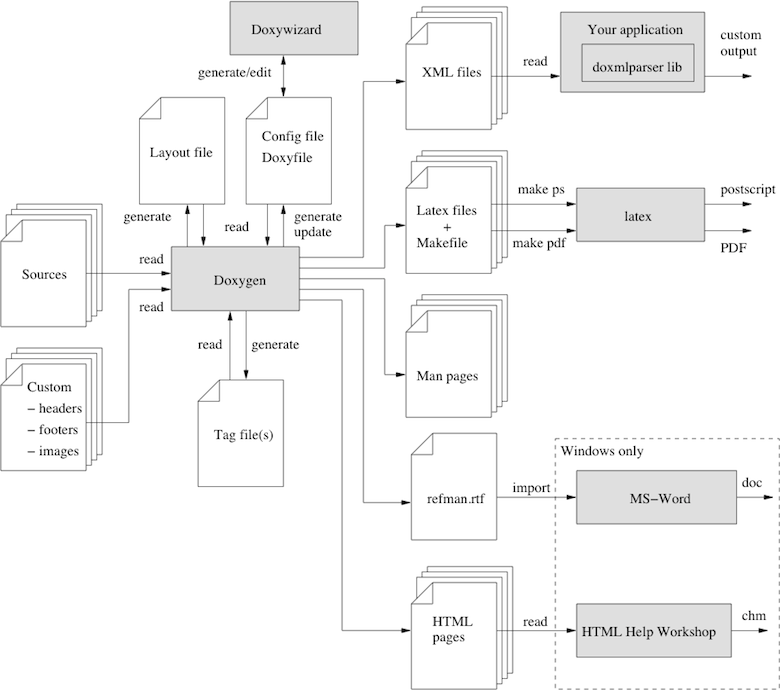
\includegraphics[width=\textwidth]{doxygenInfoflow.png} 
	\caption{Doxygen Infoflow diagramm\footcite{doxygen_main_site}}
	\label{pic:doxygenInfoflow}
\end{figure}

First a Doxygen config file, also called a \textit{Doxyfile} is generated in a project using the \textit{Doxywizard} and can be edited using this tool afterwards. 
This file is later read and updated during the generation process from \textit{Doxygen}. The layout files and tag files are also generated and used by \textit{Doxygen}
to facilitate the creation of the documentation.\\
\vspace{\baselineskip}
\textit{Sources} are the files with the actual source code, that will be part of the documentation, in them. These files are read alongside any other additional \textit{Custom}
files. For example the headers for source code, footers for the following document or images to be used in it. There are of course many other files that can be included
in order to refine the result further.\\
\vspace{\baselineskip}
Finally \textit{Doxygen} uses all this to generate documentation in the specified formats: XML, LaTex, Man, refman or HTML. \\

\subsubsection{Doxygen Configuration}
The first step in creating documentation with Doxygen is a configuration file. This can be automatically generated by the \textit{Doxywizard} with this command:

\begin{lstlisting}[language=bash]
    doxygen -g <config-file>
\end{lstlisting}

In this example \textit{<config-file>} is a stand-in for the name of the generated configuration file. There are many tags within this config file that change how 
the end result will look and what sources should be used or ignored. For example the INPUT tag specifies the location that \textit{Doxygen} will search for code and
EXCLUDE forbids it to use files contained within the given directories. After editing the file using a text editor or Doxywizard this command can be used to generate 
the documentation.

\begin{lstlisting}[language=bash]
    doxygen <config-file>
\end{lstlisting}

Doxygen normally requires the source code to be annotated in order to generate documentation, but a rough version can be made by setting the tag EXTRACT\_ALL to YES.
This will extract even the non-annotated classes and functions from the source code.

\subsubsection{Doxygen Annotation}

If the EXTRACT\_ALL tag is not enabled then the classes, functions and members within the source files need to be annotated in order to be picked up by \textit{Doxygen}
and turned into a documented section. There are many ways of signaling to \textit{Doxygen}, that you want it to produce documentation from a source. In general there
are two ways to do this:
\begin{enumerate}
    \item \textbf{Documentation within source:} In this way of annotation special comment blocks are inserted before and after parts of the source code. 
                This will cause the text within this special block to be displayed alongside the class, function, or member within the documentation.
    \item \textbf{Documentation outside source:} In this way of annotation the special comment blocks are written within a separate file and then connected 
                to the sources by way of a reference. With this method references to the source file need to be written within this distinct file.
\end{enumerate}

In \textit{Doxygen} special comment blocks are similar to C++ comments, but with extra characters in order to be picked up during generation. There are many different 
ways to define special comment blocks:\\
\vspace{\baselineskip}
\textbf{Javadoc and Qt style:} This way a special block can be definied just like a multi line comment in C++ with a special character after the first *.

\begin{minipage}{\textwidth}
\begin{lstlisting}[language=Doxygen]
    /**
     *   ... text ...
     */
\end{lstlisting}
Or:
\begin{lstlisting}[language=Doxygen]
    /*!
     *   ... text ...
     */
\end{lstlisting}
\end{minipage}
   
\vspace{\baselineskip}
\textbf{C++ comment style:} This style is similar to a C++ single line comment with an added / or ! at the begining.

\begin{minipage}{\textwidth}
\begin{lstlisting}[language=Doxygen]
    ///
    ///  ... text ...
    ///
\end{lstlisting}
Or:
\begin{lstlisting}[language=Doxygen]
    //!
    //!  ... text ...
    //!
\end{lstlisting}
\end{minipage}

\vspace{\baselineskip}
\textbf{Visible style:} This is a more clearly visible version of the previous two styles.

\begin{minipage}{\textwidth}
\begin{lstlisting}[language=Doxygen]
    /************************************
     *   ... text ...
    ************************************/
\end{lstlisting}
Or:
\begin{lstlisting}[language=Doxygen]
    //////////////////////////////////////
    ///  ... text ...
    //////////////////////////////////////
\end{lstlisting}
\end{minipage}

\vspace{\baselineskip}

In documentation outside of the source additional commands are required. At the start of the document file a special comment block needs to have the name of the
file to be documented referenced by putting a backslash or an @ symbol before the filename in the first line of the block. After that any number of other 
special comment blocks can be defined with the first line in each of them being used to reference the desired class, function, member, struct, etc. This is done by
first using the equivalent structural commands and then inserting the definition statement of the chosen object. This can be seen in this example:\\

\begin{minipage}{\textwidth}
\begin{lstlisting}[language=Doxygen]
    /*! \fn int open(const char *pathname,int flags)
        \brief Opens a file descriptor.

        \param pathname The name of the descriptor.
        \param flags Opening flags.
    */
\end{lstlisting}
\end{minipage}

In this case \textit{fn} is the structural command, which tells \textit{Doxygen} what type the object is.\\
\vspace{\baselineskip}

The other structural commands that can be seen in this example can be used in both documentation inside sources and outside sources. Using the \textit{brief} command 
is used to give a short description to the object and \textit{param} in order to signify and describe the parameters of this function.\\

\subsubsection{Doxygen Parsing}

During the documentation generation process, Doxygen parses special comment blocks and translates them into various output formats to create comprehensive 
documentation. The parser performs several key processes, culminating in the creation of documentation with Doxygen.

\begin{itemize}
    \item[] One of these processes is the conversion of Markdown writing within comment blocks into HTML, ensuring compatibility with web-based documentation platforms. This conversion improves the presentation of textual content, making it more accessible and visually appealing.
    \item[] Special commands embedded within the comment blocks are executed, allowing developers to include custom instructions or annotations. This feature empowers developers to tailor the documentation to specific project requirements, fostering flexibility and customization.
    \item[] Blank lines are handled appropriately. Paragraph separators are strategically used instead of blank lines to enhance the readability and organization of the generated documentation. This helps developers to better understand the information presented.
    \item[] Doxygen generates links to other sections of the documentation based on special comment blocks. The interlinking mechanism enables smooth navigation within the documentation, improving the user experience and promoting a cohesive understanding of the codebase.
    \item[] In situations where the output format is LaTeX, Doxygen converts HTML elements within the comment blocks into LaTeX commands. This transition ensures consistency and compatibility when generating LaTeX documents. It allows developers to choose the format that best suits their documentation needs.
\end{itemize}

\tocdata{toc}{$\rightarrow$\textit{Timon Koch}}
\subsection{Pytest}
\textbf{Author: Timon Koch}

Pytest is a testing framework for the Python programming language. It enables the creation of both simple unit tests and complex functional tests. Key features include test discovery, parameterized testing, and plugin support, making it a popular choice among Python developers. 
 
\subsubsection{Test Discovery}
The framework has the capability to automatically discover and execute test cases through a process known as 'test discovery'. By default, files that begin with 'test\_ ' or end with '\_test' are recognized as test files, although it is possible to explicitly mention other filenames. It is necessary for test method names to begin with 'test', as Test functions are identified by their names.

It is possible to either execute a specific test by indicating the corresponding identifier or execute all tests simultaneously. In the latter case, pytest will automatically detect and execute all files and functions that contain tests.  

By utilizing Pytest's plugin system, it becomes feasible to personalize and explore tests using supplementary mechanisms. The plugins available provide integration with diverse test frameworks, enabling the exclusion of particular tests or designating them for customized behaviors.

\subsubsection{Fixtures}
Fixtures are a useful feature that can help modularise and share setup code across multiple tests, resulting in improved code by increasing readability, maintainability and reusability.
They are defined as functions identified by the '@pytest.fixture' decorator. Different scopes may be specified to determine how long the fixture should last.

\subsubsection{Unit Tests}
Pytest provides compatibility with the 'unittest' testing framework. It is possible to discover and run both Pytest-style test functions and unittest test cases in the same project. This can facilitate a seamless transition between the two frameworks while leveraging the additional features provided by Pytest.

\tocdata{toc}{$\rightarrow$\textit{Christoph Fellner}}
\subsection{Pydoc}
\textbf{Author: Timon Koch}

Pydoc is a Python library and command-line tool that generates documentation from Python modules. It extracts docstrings from modules, functions, classes, and methods, and presents them in various formats, including plain text, HTML, and man pages.  Pydoc facilitates access to Python code documentation, which can aid in understanding the usage of modules, functions, and classes within a codebase. It is particularly useful for exploring Python library and module documentation without having to leave the command line or an IDE. Additionally, Pydoc can be extended and customized to support additional documentation formats or features, which can be beneficial for developers seeking to optimize their workflow. 

\tocdata{toc}{$\rightarrow$\textit{Christoph Fellner}}
\subsection{Rusqlite}
\textbf{Author: Christoph Fellner}

Rusqlite\footcite{rusqlite} emerges as a pivotal library, facilitating the seamless integration of SQLite capabilities into Rust code, akin to its analog, 
rust-postgres. This library provides a sophisticated interface, streamlining the execution of diverse database operations within the Rust programming paradigm. 
From the orchestration of table creation and data insertion to the intricacies of data querying, rusqlite empowers developers with a versatile toolset for 
database manipulation directly within their Rust codebase.

The decision to adopt rusqlite in our specific use case is underpinned by a meticulous consideration of three critical factors:

\begin{enumerate}
    \item \textbf{Portability:} SQLite's commendable attribute of cross-platform compatibility across diverse operating systems assumes paramount importance in 
    our context at RECT. Given the heterogeneous nature of small controllers operating within our system, the ability to seamlessly deploy SQLite databases 
    across different platforms becomes imperative for maintaining operational uniformity and efficiency.
    
    \item \textbf{Configuration:} In stark contrast to database systems that necessitate intricate setup procedures, SQLite obviates the need for complex 
    configurations. The simplicity inherent in working with SQLite aligns seamlessly with our operational requirements. The nominal requirement for a limited 
    number of tables further amplifies the pragmatic appeal of SQLite. In contrast to configuring a database on each controller, the minimal setup overhead 
    consolidates SQLite as the optimal choice for our streamlined operational demands.
    
    \item \textbf{Local:} SQLite distinguishes itself by eschewing the necessity for an external server or intricate installations. Its self-contained package 
    encapsulates all requisite features within a local environment. This intrinsic localization resonates with the operational ethos at RECT, aligning with the 
    need for an efficient and autonomous database solution without the encumbrance of external dependencies.
\end{enumerate}

In our specific instantiation, rusqlite is strategically employed for the persistent storage of the config.json file, a repository of vital data concerning 
available connections. The judicious selection of rusqlite in this context is grounded in its inherent advantages. The utilization of rusqlite markedly enhances 
the expediency and security of data access compared to traditional file-based retrieval mechanisms. This methodological choice contributes not only to the 
enhanced performance of our system but also underscores the commitment to preserving the integrity and reliability of configuration data, pivotal to the seamless
functionality of our application within the broader scientific and technological landscape.

\tocdata{toc}{$\rightarrow$\textit{Christoph Fellner}}
\subsection{Serde}
\textbf{Author: Christoph Fellner}

Serde\footcite{serde} emerges as a pivotal tool in the Rust programming ecosystem, dedicated to the efficient and generic serialization and deserialization 
(\textbf{ser}ialization/\textbf{de}serialization) of data structures. Offering a robust foundation for these operations, Serde plays a crucial role in optimizing
the handling of data structures within the Rust programming paradigm. For a comprehensive overview of Serde, interested readers can refer to the detailed 
documentation available at \href{https://serde.rs/}{https://serde.rs/}.\newline

The salient features of Serde become particularly evident in its capability to facilitate the seamless deserialization of JSON files with efficiency and 
simplicity. This functionality proves invaluable in our context, where the utilization of data from the config.json file is an integral part of our program. 
Serde streamlines this process, enabling us to incorporate the data effortlessly into our program with just a few lines of code.\newline

By leveraging Serde, we engage in a streamlined deserialization process wherein the data from the JSON file is efficiently transformed into a custom Rust 
structure. This bespoke structure, tailored to our specific needs, enables us to harness the deserialized data seamlessly within our program. The utilization of
Serde thus transcends mere deserialization, providing us with a powerful and adaptable mechanism to work with the data in a meaningful and efficient manner.\newline

In essence, the incorporation of Serde into our workflow is not merely a technical choice but a strategic one, driven by the need for optimized data handling 
and seamless integration of external data sources. Through Serde, our program gains a robust and flexible capability to decode JSON files, thereby enhancing the
overall efficiency and maintainability of our Rust-based application.

\tocdata{toc}{$\rightarrow$\textit{Christoph Fellner}}
\subsection{Tokio}
\textbf{Author: Christoph Fellner}

Tokio\footcite{tokio} serves as a pivotal asynchronous runtime for Rust, addressing the intricacies of asynchronous code execution in the language. In Rust, 
asynchronous code does not inherently execute independently; rather, it necessitates the use of a runtime like Tokio to effectively function. For an in-depth 
exploration of Tokio and its capabilities, readers are encouraged to delve into the detailed tutorial available at 
\href{https://tokio.rs/tokio/tutorial}{https://tokio.rs/tokio/tutorial}.\newline

The selection of Tokio as our asynchronous runtime is underpinned by several compelling reasons. Chief among them is Tokio's status as the preeminent and widely
adopted runtime for asynchronous Rust code. Its widespread usage within the Rust community attests to its robustness and reliability in facilitating asynchronous
programming paradigms.\newline

Moreover, Tokio's popularity is bolstered by the abundance of tutorials and educational resources available, making it approachable for developers seeking to 
harness the power of asynchronous programming in Rust. The simplicity and accessibility of Tokio's interface contribute to its widespread adoption, enabling 
developers to swiftly grasp and implement asynchronous patterns in their codebase.\newline

One of the key advantages of Tokio lies in its ability to execute multi-threaded asynchronous code safely. This capability is crucial in scenarios where 
parallelism and concurrency are essential, such as in web servers or applications handling numerous concurrent tasks. Tokio's adept handling of multi-threaded 
asynchronous code ensures the efficient execution of tasks without compromising safety or introducing race conditions.\newline


In summary, our decision to embrace Tokio as the asynchronous runtime for our Rust project is grounded in its status as the leading runtime in the Rust 
ecosystem, coupled with its user-friendly design and robust support for multi-threaded async code execution. This strategic choice positions us to harness the 
full potential of asynchronous programming in Rust, ensuring the responsiveness and scalability of our application.

\begin{verbatim}
#[tokio::test(flavor = "multi_thread", worker_threads = 2)]
async fn client_test(){ 
    let ser = test_server::run_server();
    println!("Server started");
    let cl = test_client::client_test();
    println!("Client started");

    tokio::select! {
        biased; 
        _ = ser => panic!("server returned first"),
        _ = cl => (),
    }           
}
\end{verbatim}

Using Tokio makes it possible to run multiple async functions at the same time. In the example above we start a server and a client and then wait for the first one to finish. 
This is done using the tokio::select! macro. The macro takes a list of futures and waits for the first one to finish. In our case we want to wait for the client to finish 
first, so we panic if the server finishes first. If the client finishes first we just return. Any occoring Errors are cathed and returned as Result.
The two functions \verb+run_server+ and \verb+client_test+ are both async functions. The server function is a simple echo server, that waits for a message from the client and 
then sends it back. The client function sends a message containing an url and a vote to the server and then waits for the response. Server and Client are connected via a gRPC 
connection. 

\tocdata{toc}{$\rightarrow$\textit{Christoph Fellner}}
\subsection{Tokio Rusqlite}
\textbf{Author: Christoph Fellner}

Tokio Rusqlite\footcite{tokiolite} stands as an innovative library at the intersection of Tokio and Rusqlite, synergizing their functionalities to enable 
asynchronous database interactions. This library represents a strategic amalgamation, providing developers with the capability to leverage Rusqlite seamlessly 
within an asynchronous programming paradigm facilitated by Tokio.\newline

The amalgamation of Tokio and Rusqlite in Tokio Rusqlite addresses the growing demand for asynchronous database operations in Rust. By integrating Tokio's 
asynchronous runtime with Rusqlite's capabilities, this library empowers developers to perform database operations without blocking the execution of other tasks.
This is particularly advantageous in scenarios where responsiveness and concurrency are paramount.\newline

Key features of Tokio Rusqlite include the ability to execute Rusqlite operations asynchronously, allowing for non-blocking interactions with SQLite databases. 
Asynchronous operations are vital in applications that require efficient handling of concurrent tasks, such as web servers, where multiple requests may be 
processed simultaneously.\newline

The seamless integration of Tokio Rusqlite into our development stack augments the versatility of Rusqlite by enabling asynchronous database operations. This is 
especially valuable in scenarios where responsiveness and scalability are critical factors. Leveraging Tokio Rusqlite in our project equips us with a robust 
solution for handling database interactions in an asynchronous manner, aligning with contemporary trends in Rust programming and distributed system 
architectures.

\tocdata{toc}{$\rightarrow$\textit{Christoph Fellner}}
\subsection{Tonic}
\textbf{Author: Christoph Fellner}

Tonic\footcite{tonic}, a Rust library that embodies the principles of gRPC, distinguishes itself with a keen focus on high performance, interoperability, and 
flexibility. Its seamless integration with the asynchronous paradigm, particularly its compatibility with Tokio, positions Tonic as a versatile tool for 
developing efficient and responsive distributed systems.\newline

The synergy between Tonic and Tokio is a noteworthy feature, as Tonic is crafted to align seamlessly with Tokio's asynchronous model. This compatibility not 
only enhances the performance of asynchronous Rust code but also simplifies the integration of Tonic into existing Tokio-based projects. Leveraging async/await 
functionality, Tonic facilitates a synchronous coding style in an asynchronous environment, making it a natural fit for projects utilizing Tokio.\newline

A distinctive aspect of Tonic lies in its support for gRPC, a high-performance remote procedure call (RPC) framework. Tonic employs Protocol Buffers to describe 
interfaces, providing a language-agnostic and efficient means of defining the structure of data. This approach not only enhances interoperability but also 
allows for the generation of necessary Rust code based on the defined Protocol Buffers, automating a significant portion of the development process.\newline

The utilization of Tonic in our project streamlines the definition of interfaces by leveraging Protocol Buffers. This enables us to articulate our interface 
specifications in a clear and concise manner, and Tonic then takes care of the Rust code generation, reducing manual effort and potential errors.\newline

In essence, Tonic serves as a powerful tool in our technology stack, providing a performant and flexible implementation of gRPC for Rust. Its compatibility with 
Tokio, support for async/await, and seamless integration with Protocol Buffers contribute to the development of robust and efficient distributed systems. By 
choosing Tonic, we aim to leverage its capabilities to enhance the performance, interoperability, and maintainability of our Rust-based projects.\newline

The example for Tokio above uses the Tonic library to convert the following Protocol-Buffer-file into Rust code, in order to use it in the client and server 
functions as Service.

\begin{minipage}{\textwidth}
\begin{lstlisting}[language=ProtoBuf]
syntax = "proto3";
package voting;
        
service Voting {
    rpc Vote (VotingRequest) returns (VotingResponse);
}
        
message VotingRequest {
    string url = 1;
        
    enum Vote {
        UP = 0;
        DOWN = 1;
    }
    Vote vote = 2;    
}
        
message VotingResponse {
    string confirmation = 1;
}
\end{lstlisting}
\end{minipage}

In order to translate the Protocol Buffer into Rust code we use the \verb+include_proto!+ function from the Tonic library. This function takes the path to the 
Protocol-Buffer-file and generates the Rust code for the Service.

\tocdata{toc}{$\rightarrow$\textit{Christoph Fellner}}
\subsection{Docker}
\textbf{Author: Christoph Fellner}

Docker\footcite{docker} serves as an indispensable tool in modern software development, offering a containerization solution that facilitates the efficient 
execution of diverse applications within isolated environments known as containers. These containers, encapsulating applications and their dependencies, operate 
independently, enabling the concurrent execution of multiple containers on a single host system. The versatility of Docker extends from lightweight services 
like echo servers to complex web applications, making it a versatile choice for a spectrum of development and deployment scenarios.\newline

One of Docker's compelling use cases is the encapsulation of databases within containers. This capability enables the creation of portable and reproducible 
database environments, fostering ease of testing, development, and even benchmarking. In our specific use case, Docker proved instrumental in benchmarking 
different databases, allowing us to evaluate and identify the most suitable database for our application's requirements.\newline

Docker's open-source nature and compatibility across major operating systems contribute to its widespread adoption. Its availability on diverse platforms 
empowers developers to create consistent environments, irrespective of the underlying infrastructure. This feature is particularly advantageous in scenarios 
where multiple applications need to coexist on the same machine, as Docker mitigates compatibility concerns and ensures the isolation of applications from the 
local infrastructure.\newline

The ability to isolate applications from the host system's infrastructure is a key feature of Docker. This isolation not only enhances compatibility but also 
simplifies the deployment process. Developers can confidently run multiple applications on a single machine without the fear of conflicts or compatibility 
issues, streamlining the development and testing phases.\newline

In summary, Docker's role in our project extends beyond conventional application development and deployment; it serves as a pivotal tool for benchmarking 
databases. Its containerization approach, coupled with the ability to create reproducible environments, positions Docker as a valuable asset in our quest to 
identify the optimal database solution for our specific use case. The open-source nature and cross-platform compatibility further solidify Docker's standing as 
a cornerstone technology in contemporary software development and deployment practices.

\filbreak

	\chapter{Implementation}

\section{CommLib}
\textbf{Author: Jeremy Sztavinovszki} 
The Communication Library, or CommLib for short is the part of the RECT stack, that handles all of the communication between the hosts over traditional protocols, like TCP, UDP and BLE.
This requires it to be especially performant. In order to avoid premature optimization however, the first part of this section on the implementation of the CommLib will only cover the first versions
of the code written to get the Library to work. After the first implementation there will be benchmarks and some profiling, in order to get a grasp on which aspects of the library need to be
optimized. The second section will then cover how these results were incorperated into designing a more polished version of the CommLib.

\subsection{Setting up the Library} 
The first steps of setting up the library are more or less the same as in any other rust project. First the project is initialized with \verb+cargo new --lib <rust-name>+. This creates a
new folder with the name specified in \verb+<library-name>+ and generates some files like Cargo.toml and src/main.rs. After this step is done the needed libraries for RECT are added to the
project through \verb+cargo add <dependency-name> -F <dependency-name>/<feature-name>+ these dependencies are the pulled and built by cargo (Rust's build tool) upon the initial build of the
project. The first iteration of the project then had the following dependencies:

\begin{itemize}
	\item tokio
	\item bluer
	\item anyhow
\end{itemize}

All in all the commands used to generate the CommLib project and install all dependencies looked like this:
\newline
\begin{minipage}{\textwidth}
	\begin{lstlisting}[language=bash, caption=Setup Commands for CommLib]
		cargo new --lib CommLib && cd CommLib
		cargo add tokio bluer anyhow -F tokio/full,bluer/full
		cargo build
	\end{lstlisting}
\end{minipage}

\subsection{First Implementation}
The first part of the implementation that was tackled was to create an abstraction layer over the existing protocols that RECT uses.
in order to have a nice and clean interface to work with and to avoid having to implement each feature separately for the
protocols. Of course, there was a bit of a problem with UDP because it is not meant to send structured data, so there is no feature parity between TCP and BLE.
between TCP and BLE and UDP in this respect, and UDP is only used to send unstructured data streams. To encapsulate the structured and unstructured data sent over the
and unstructured data sent over the common interface, there needs to be a way to convert the data, whether structured or not, into and from bytes in a way that is performant and has minimal overhead.
and has minimal overhead. In order to meet the above requirements, the following structure has been implemented.
 
\subsubsection{Messages and Packets}
% TODO Write about the packets and messages and maybe do a nice graphic.
% TODO find cite for TCP and UDP MTU 
The first thing taken into consideration for designing a data and class structure that is able to be sent over all of the protocols is the MTU's of the different protocols. 
For TCP and UDP the MTU, or maximum transmission unit, is defined by the Maximum Segment Size Option (MSS), which is technically limited to 65535 bytes (64KB), but as defined
in RFC 2675 \footcite{rfc2675} an MSS value of 65535 is defined to be interpreted as infinity and to be determined by Path MTU Discovery \footcite{rfc9293}. For BLE the MTU is 
defined by the L2CAP and can be anywhere from 23 to 65535, but the packet is fragmented and recombined by the L2CAP for transmission, which practically makes it infinite. % TODO find out why ble book cant be cited 

Another requirement for the interface was to be able to encapsulate the mechanism of sending a request to a peer and receiving a response. 
To do this, a pair of messages was implemented. This pair of messages, aptly named Request and Response, contains the data needed to make this work. This means 
that the request contains information about what topic to call on the remote machine, the data needed to fulfil that call, and an identification of the calling process, 
while the response contains the returned data and the ID of the client to which it should be returned. This identification is used to avoid confusion as to which process the data should be returned to, 
for example, when multiple processes are requesting data from the same remote service.

The identification mechanism used in the above case of sending data to a single recipient can also be adapted to send messages to multiple recipients.
The only adaptation required for the requesting and responding application to be able to send and receive broadcasts is to create a proxy object on the receiving side that acts as a single 
receiver to receive the data for multiple connections and then forward that data to all subscribing processes.  

The last use case covered by CommLib is the sending of a continuous stream of data. An example of this would be a sensor continuously sending data. To avoid the overhead of sending values over
protocols used in CommLib, it was decided to require a separate interface, e.g. a socket, that is used only for streaming the described data. This means that when the receiving side
is establishing a connection, it only needs to look at the identifier, e.g. the IP address, of the connected peer to decide which process to pass the data to, instead of reading a connection 
name from the packet sent, minimising the size of the packets that need to be sent. 

% TODO Write about the connection manager and also program that stuff
\subsubsection{The ConnectionManager}
The most important component in the whole CommLib is the ConnectionManager. It is a singleton object, which as the name would suggest manages all of the needed and used connections that are
requested by the client programs. Because the ConnectionManager is a singleton and because it must be able to handle being in concurrent execution environments the Rust borrow-checker has very
special requirements for how it is accessed. To meet these requirements the static variable holding the ConnectionManager singleton has needs to be wrapped in several objects to ensure it is
thread-safe, as well as making sure, that it is initialized and freed, when there are no references left to its smart-pointer. 

\begin{lstlisting}[language=Rust]
	pub static CONNECTION_MANAGER: Lazy<Arc<Mutex<ConnectionManager>>> =
	    Lazy::new(|| Arc::new(Mutex::new(ConnectionManager::new())));
\end{lstlisting}
Which leads to the above code, which has specifies, that the ConnectionManager is wrapped in the following types.

\begin{itemize}
	\item Lazy. This type allows any object held by it to be initialized only once and only when it is first called upon \footcite{once-cell-lazy}
	\item Arc. Arc stands for atomic reference counter and is a type of smart-pointer used in rust, when pointers need to be thread safe \footcite{rust-arc}
	\item Mutex. The mutex ensures, that only one process at a time can hold a reference to the held object in order to prevent issues such as race-conditions \footcite{tokio-mutex}
\end{itemize}

Any application using the CommLib needs to interact with this object in order to be able to use the communication methods provided by the library. But what functionality does the ConnectionManager provide?

\begin{itemize}
	\item Setting a connection to a database, which is used to read the connections configured by the clients.
	\item Receiving streams, requests and responses through any of the configured connections.
	\item Sending streams, requests and responses through any of the configured connections.
	\item Initiating an update of the connections, which checks changes in the configuration found in the database and the connections, that are currently active in the ConnectionManager.
\end{itemize}

% TODO Pretend you didn't already make everything railway programming and it still crashes because of stupid things.

\subsection{Profiling and Benchmarking}

\subsection{Polishing}

\subsection{Documentation}

\section{RECT Database}
\textbf{Author: Christoph Fellner}

\subsection{Why SQLite?}
The choice of a database system is a critical decision in the development of any application, and for RECT, the decision to use SQLite as the backend database 
is grounded in a thoughtful consideration of specific requirements tailored to the nature of small controllers.\newline

Given the diverse landscape of database systems, each with its unique set of advantages and drawbacks, a comprehensive evaluation of options is imperative. 
RECT's emphasis on catering to small controllers immediately guides the criteria for selecting a suitable database. Two key considerations emerge prominently: 
memory efficiency and self-containment.\newline

Small controllers typically operate within constrained resources, making memory efficiency a paramount concern. SQLite, renowned for its lightweight nature and 
minimal memory footprint, aligns seamlessly with this requirement. Its design prioritizes efficiency, ensuring optimal performance even in resource-limited 
environments.\newline

The self-contained nature of SQLite further contributes to its suitability for RECT's use case. Unlike some database systems that necessitate complex setup 
procedures and external dependencies, SQLite operates as a standalone, serverless database engine. This simplicity not only facilitates ease of use but also 
aligns with the desire to avoid intricate configurations. RECT benefits from a database solution that is straightforward to use and configure, enabling a 
seamless integration into the development workflow.\newline

While the focus on memory efficiency and self-containment narrows down the pool of potential databases, SQLite emerges as an optimal choice that strikes a 
balance between these requirements. The careful consideration of these factors positions SQLite as a reliable and pragmatic choice for RECT, providing the 
necessary functionality without introducing unnecessary complexity.\newline

In conclusion, the selection of SQLite for RECT's backend database is a result of a meticulous comparison of different options, with a keen focus on the 
specific needs of small controllers. The prioritization of memory efficiency, self-containment, and ease of use collectively affirm SQLite as the ideal database 
solution, ensuring optimal performance and simplicity in the context of RECT's development environment.

\subsubsection{SQLite}
SQLite\footcite{sqlite} stands out prominently as a frontrunner when it comes to selecting a memory-efficient database, and for good reasons. As a small, fast, 
and serverless database engine, SQLite aligns perfectly with the requirements of applications like RECT, particularly those designed for small controllers.\newline

The serverless nature of SQLite is a noteworthy feature. Unlike some database systems that necessitate a separate server process for operation, SQLite operates 
in a self-contained manner. This characteristic not only simplifies deployment and configuration but also contributes to its efficiency and suitability for 
resource-constrained environments.\newline

\paragraph{History}
Originally developed in the year 2000 by D. Richard Hipp for the US Army, SQLite has evolved into an open-source database engine. Its implementation in the C 
programming language renders it highly portable, allowing it to run seamlessly on a myriad of platforms. This broad compatibility makes SQLite an excellent 
choice for applications that need to be deployed across diverse environments.\newline

\paragraph{Compatibility with Rust}
The compatibility between SQLite and Rust is facilitated through the rusqlite library, providing a native and ergonomic interface for Rust developers to 
interact with SQLite databases. This seamless integration ensures that the benefits of SQLite, such as its speed and efficiency, can be harnessed effortlessly 
within Rust projects.\newline

Moreover, SQLite offers the flexibility to store the database in memory, enabling rapid access and retrieval of data. The asynchronous access to SQLite 
databases further enhances its versatility, allowing applications like RECT to efficiently manage and interact with data in an asynchronous programming paradigm.\newline

In essence, SQLite's combination of speed, efficiency, serverless operation, and broad platform compatibility positions it as an ideal choice for applications 
that prioritize memory efficiency. For RECT, SQLite, with its inherent qualities and compatibility with Rust through rusqlite, emerges as a robust and fitting 
solution for the backend database, contributing to the overall efficiency and performance of the application.

\subsubsection{PostgreSQL}
Postgres\footcite{postgres}, also known as PostgreSQL, stands as a widely adopted backend database for web applications and websites. Renowned for its robust 
features and scalability, PostgreSQL operates on a client/server architecture, where the database is managed by a dedicated server process. This architecture 
allows multiple clients to interact with the database concurrently, even when accessing the same data simultaneously. The inherent support for handling multiple 
clients makes PostgreSQL particularly well-suited for scenarios where asynchronous access to the database from multiple threads is crucial.\newline

\paragraph{History}
The origins of PostgreSQL trace back to the Berkeley Computer Science Department at the University of California in 1986. Initially named Postgres, the project 
evolved over time and eventually became known as PostgreSQL, although the colloquial shortening to Postgres is still common. In 1996, the project transitioned 
to an open-source model, relying on the contributions of a dedicated group of volunteers for maintenance and improvement. Operating seamlessly on major 
operating systems, PostgreSQL has garnered a reputation for its reliability and adherence to standards.\newline

\paragraph{Compatibility with Rust}
In the realm of Rust, PostgreSQL finds compatibility through the rust-postgres library, which provides a native interface for Rust developers to interact with 
PostgreSQL databases. The integration of Rust and PostgreSQL is further optimized for asynchronous programming through the tokio-postgres library. This library, 
built on top of Tokio, enhances the performance of asynchronous interactions with PostgreSQL databases via Rust, making it well-suited for modern, concurrent 
application scenarios.\newline

The client/server architecture of PostgreSQL, coupled with its robust Rust libraries, positions it as a formidable choice for applications that require a 
backend database with support for concurrent access and asynchronous operations. While it may have started as a project nearly four decades ago, PostgreSQL 
continues to evolve and thrive, maintaining its relevance in the dynamic landscape of web development and database management.

\subsubsection{MySQL}
MySQL\footcite{mysql} has established itself as a heavyweight in the realm of backend databases, with giants like YouTube, Facebook, and Twitter relying on its 
robust capabilities. Widely utilized for storing data from web services, MySQL operates on a client/server architecture similar to PostgreSQL, featuring a 
singular server process managing the database and facilitating access for multiple clients.\newline

\paragraph{History}
The MySQL project traces its roots back to 1994 when Michael Widenius and David Axmark initiated its development. Initially conceived as a fork of the mSQL 
database, MySQL underwent a significant transformation and was eventually rewritten from scratch. Since 2010, MySQL has been under the development umbrella of 
Oracle. While the project remains open-source, Oracle also offers an enterprise version of MySQL with additional features and support.\newline

In response to concerns about the direction of MySQL's development under Oracle, the original developers embarked on a new venture called MariaDB. This project 
represents a fork of MySQL and maintains full compatibility with its predecessor. The availability of MariaDB provides users with an alternative that adheres 
to the principles of open-source development.\newline

\paragraph{Compatibility with Rust}
For Rust developers seeking to interface with MySQL, the mysql library, complemented by an extension called \verb+mysql_async+, offers a convenient and native 
Rust interface. The \verb+mysql_async+ library, built on the Tokio framework, specifically caters to asynchronous client access, aligning with modern 
programming paradigms that emphasize concurrent and non-blocking operations.\newline

In summary, MySQL's widespread adoption by major players in the tech industry underscores its reliability and scalability as a backend database. The project's 
history, marked by its evolution under different entities, has given rise to alternative options such as MariaDB. The existence of Rust libraries like mysql 
and \verb+mysql_async+ further enhances MySQL's accessibility and usability within the Rust programming ecosystem, enabling developers to seamlessly integrate 
MySQL into their applications.

\subsubsection{Comparison}
The table provides a concise comparison of key features among SQLite, PostgreSQL, and MySQL, shedding light on their architectural, compliance, support, and 
use-case distinctions:

\begin{center}
    \begin{tabular}{ | m{3cm} | m{4cm}| m{4cm} | m{4cm} | } 
      \hline
      Features & SQLite & PostgreSQL & MySQL \\ 
      \hline
      Architecture & File Based (Self-contained) & Client/Server & Client/Server \\ 
      \hline
      ACID Compliance & Always & Always & Only with InnoDB and NDB Cluster storage engines \\ 
      \hline
      In-memory Support & Yes & No & Yes \\
      \hline
      Editions & Community (Free) with option of pro support & Community with option of commercial support & Community, Standard, and Enterprise \\
      \hline
      Popular Use-cases & Low-Medium Traffic Websites, IoT and Embedded Devices, Testing and Development & Analytics, Data Mining, Data Warehousing, Business Intelligence, Hadoop & Web Sites, Web Applications, LAMP stack, OLTP-based applications \\
      \hline
      Key Customers & Adobe, Facebook, and Apple & Cloudera, Instagram, and ViaSat & GitHub, Facebook, and YouTube \\
      \hline
    \end{tabular}
\end{center}

This comparison underscores the diverse strengths and use cases of each database system. SQLite's file-based, self-contained architecture makes it suitable for 
low to medium traffic websites, embedded devices, and development environments. PostgreSQL, with its client/server architecture and robust feature set, caters 
to analytics, data mining, warehousing, and business intelligence needs. MySQL, available in various editions, is widely employed in web applications, LAMP 
stack environments, and OLTP-based applications. Each database system has its own unique advantages, making the selection contingent on the specific 
requirements and scale of the intended use.\newline

After we looked into the three possiblyties mentioned above we created an enviroment to benchmark the different databases. We used docker to create a container for each 
database and then ran a benchmark test on each of them. The benchmark test was a simple test that inserted 1000 rows into a table and then read them again. The benchmark is
purposefully simple, because we won't be using the database for complex queries. More about the benchmark tests can be found \href{tests.tex}{here}.

\subsection{Database Structure}

The RECT Database is designed like \ref{fig:db-architecture}. This is a Entity Relationship Diagram (ERD) that shows the structure of the database. The database implements a
classic star schema, with the connections table as the center of the star. The connections table is linked to the client, method and address tables.

\begin{figure}
	\centering

	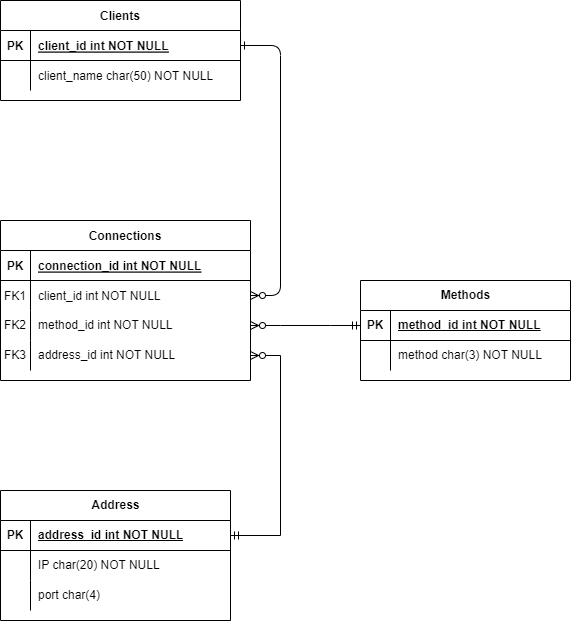
\includegraphics[width=\textwidth]{img/RECT-erd}

	\caption{Database Architecture of RECT.}
	\label{fig:db-architecture}
\end{figure}



The RECT database is structured according to the widely adopted star model, providing a robust framework for efficiently managing connection data. Comprising four distinct 
tables, namely connections, client, method, and address, this database architecture ensures comprehensive organization and accessibility of critical information.\newline

The connections table serves as a central hub, linking to the other three tables through their respective IDs and storing unique identifiers for each connection. 
Meanwhile, the client table houses data pertaining to the clients associated with specific connections, facilitating targeted access to connection information. In the 
method table, precisely three objects—BLE (Bluetooth Low Energy), TCP (Transmission Control Protocol), and UDP (User Datagram Protocol)—are stored, representing the 
available connection types within the RECT ecosystem. Additionally, the address table stores essential network information, including IP addresses and ports, with the 
provision for a null port value in instances where the connection method is BLE.\newline

By adopting this schema, the RECT database optimizes accessibility to connection data for clients by establishing seamless linkages between tables. Leveraging the Rusqlite
library, the backend components can efficiently query and retrieve pertinent information, enabling effective communication over the designated connections. Moreover, this 
database structure facilitates the extraction of various insights and metrics, empowering users to select and analyze data such as:

\begin{itemize}
  \item[] How many BLE, TCP or UDP connections are available?
  \item[] All connections of a specific client.
  \item[] All clients that have a specific connection.
  \item[] All connections that are available.
  \item[] How many connections are available in total?
  \item[] Are there more connections to the same client?
\end{itemize}

\subsection{Database usage}

The RECT Database serves as a pivotal resource accessible not only to the Rust Interface but also to the entirety of the backend infrastructure within the RECT stack. 
Acting as the backbone for data management, the Rust Interface undertakes the essential task of configuring the database, a process that includes the insertion of data 
sourced from the JSON file into its tables. This data encompasses a comprehensive inventory of available connections tailored specifically for the local RECT Client system.
Each connection within this dataset is meticulously characterized by a unique identifier, a designated communication method (be it BLE, TCP, or UDP), and a corresponding 
address composed of an IP address and port number.\newline

Upon completing the database setup and population with pertinent connection data, the backend components of the RECT stack rely on this repository to establish and manage 
communication channels. However, before the backend can effectively harness the capabilities of the database, the Rust Interface must first initialize the database setup 
and meticulously inject the JSON-derived information. Following this preparatory phase, the Interface seamlessly facilitates backend access to the database via the CommLib,
thereby ensuring a streamlined pathway for communication. Subsequently, armed with access to this centralized database, the backend components adeptly navigate and utilize
the provided connections to facilitate efficient communication processes tailored to the demands of the RECT ecosystem.

\section{Rust Interface}
\textbf{Author: Christoph Fellner}
One of the main sections of the RECT project is the Rust Interface. The Rust Interface is the part of the RECT stack that is responsible for the communication between 
the different parts of the stack. That means that the Rust Interface is responsible for the communication between the CommLib and the RECT Database. The RECT Database is 
part of the Rust Interface, it stores Data about all available RECT connections. The Rust Interface also communicates with the Python Service and the C++ Service. So 
basically the Rust Interface it responsible for the communication between the frontend and the backend of the RECT stack.\newline

In order to achieve this functionality the first step was to create a Rust module for gRPC communication. The gRPC communication is done with the help of the tonic library.
The tonic library is a gRPC library for Rust, which is based on the tokio library. The tokio library is a runtime for writing reliable asynchronous applications with Rust.
The gRPC module is responsible for the communication between the Rust Interface and the Python Service and the C++ Service. The gRPC module is also responsible for the 
communication between the Rust Interface and the CommLib.\newline 

The second step was to create a module for the RECT Database. The RECT Database is a in-memory SQLite database. The module uses the rusqlite library with the addition of
the tokio-rusqlite library. The tokio-rusqlite library is a asynchronous version of the rusqlite library. The Rust Interface implements the RECT Database, creates the 
necessary tables and provides the necessary functions to communicate with the database. The module is also responsible for the inserts of the available connections from a
JSON file into the database. The JSON file is created by the frontend and contains all available connections for the RECT stack.\newline

For the second step to work the Rust Interface also needs to be able to read the JSON file. The JSON file is read by another module of the Rust Interface. The module uses
the serde library to read the JSON file. The serde library is a framework for serializing and deserializing Rust data structures efficiently and generically. The module 
defines suitable structures for the data strored in the JSON file and then reads the file and stores the data in the defined structures. The database module then takes
this data and stores it in the RECT database.\newline

With these modules completed the Rust Interface is able to communicate with the CommLib, the Python Service and the C++ Service. In conclusion, the Rust Interface plays a 
crucial role within the RECT project, facilitating communication between various components of the stack. Through the implementation of modules for gRPC communication and 
the RECT Database, the Rust Interface ensures seamless interaction between the frontend and backend elements. Leveraging libraries such as tonic, tokio, rusqlite, and 
serde, the interface achieves reliable and efficient communication, handling tasks such as database management and data serialization effectively. Overall, the Rust 
Interface serves as a vital bridge, enabling smooth operation and integration within the RECT stack.

\section{Rust Service}
\subsection{Documentation}

\section{C++ Implementation}
\textbf{Author: Maximilian Dragosits}
The C++ Implementation is one of the two outward facing components of the RECT stack. Alongside the Python Implementation 
it serves as a library in order for developers to be able to create robots, that are able to communicate with each other, much
easier then before. This is accomplished by abstracting most of the complexities of gRPC behind the \textit{Rectcpp} class. 

The class only needs to be initialized with IP-Addresses for the different services that it offers and be given the IP of 
another of its kind and then it should be a simple act of using the predefined methods within the class in order to 
effortlessly communicate with other robots or devices running this or the Python frontend implementation.

\subsection{Rectcpp class}
\subsection{Documentation}

\section{Python Implementation}

\subsection{Documentation}

\section{Implementation Comparison}

\filbreak

	%\chapter{Experiment 1}
\textbf{} 

\filbreak
	%\chapter{Lessons learned}

\textbf{Author: } 

\filbreak
	%\chapter{Experiment 2}

\textbf{Author: } 


\filbreak
	\chapter{Tests}

\textbf{Author: Timon Koch}

\section{Specialized Benchmarks and Tests}
\subsection{Serialization and Compression}

\section{Optimization}
\subsection{Compression}
\textbf{Timon Koch}

By reducing the size of data, compression saves storage space, speeds up data transmission over networks and minimises bandwidth requirements, resulting in cost savings and improved operational efficiency. In addition, compressed data is easier to manage, share and access across platforms and devices. 

\subsubsection{Deflate}
The Deflate algorithm is a widely used method of lossless data compression. It achieves compression by eliminating redundancy in the input data through a combination of LZ77 and Huffman coding techniques, making it an efficient and versatile compression method used in various applications.

In the first step, LZ77 identifies repeated substrings in the data and replaces them with references to previous occurrences, thereby reducing redundancy. This is followed by Huffman coding, which assigns shorter codes to more frequent symbols and longer codes to less frequent symbols, further compressing the data

\subsubsection{ZSTD}
ZSTD, short for Zstandard, is a high performance data compression algorithm developed by Facebook. It is designed to provide both fast compression and decompression speeds while achieving excellent compression ratios, making it suitable for a wide range of applications.

ZSTD uses a combination of advanced compression techniques, including a dictionary-based approach, context modelling and entropy coding. It dynamically builds and updates dictionaries during compression to improve compression efficiency by identifying and exploiting patterns in the data.

\subsubsection{GZIP}
GZIP, short for GNU Zip, is based on the Deflate algorithm. While it's optimised for speed, GZIP also provides reasonably good compression ratios, making it a popular choice for applications where both speed and compression efficiency are important.

GZIP typically offers several levels of compression, allowing users to trade off compression ratio and speed according to their needs. Lower compression levels prioritise faster processing times, while higher levels prioritise better compression ratios at the expense of speed.

\subsection{Buffering}

\subsection{Serialization Formats}
\textbf{Author: Timon Koch}

\subsubsection{JSON}
JSON (JavaScript Object Notation) is a lightweight data-interchange format that is easy for humans to read and write and easy for machines to parse and generate. It is based on a subset of the JavaScript programming language.

JSON consists of key-value pairs, where keys are strings and values can be strings, numbers, arrays, objects, booleans, or null. It is highly versatile and widely supported across various programming languages and platforms.

\subsubsection{YAML}
YAML (YAML Ain't Markup Language) is a data serialisation format commonly used for configuration files, data exchange, and specifying data structures in a clear, concise, and readable manner. It uses indentation and whitespace to represent data hierarchies, making it visually intuitive and easy to understand.

YAML supports multiple data types, including scalars (strings, numbers, booleans), sequences (arrays or lists), and mappings (key-value pairs). It also allows for comments, making it useful for annotating configurations and documentation.

\subsubsection{Protobuf}
Protocol Buffers (protobuf) is a method of serialising structured data developed by Google. Designed to be efficient, portable and easy to use, it provides a platform-neutral way to encode data for communication between systems or for persistent storage.

Protobuf defines a schema for data structures using a language-agnostic interface description language (IDL). This schema describes the structure of the data in a concise and platform-independent manner. From this schema, Protobuf compilers generate code in various programming languages, allowing developers to easily work with the defined data structures.

\subsubsection{Bincode}
Bincode is a binary serialisation format designed for use with the Rust programming language. It allows the serialisation of Rust data structures into a compact binary representation that can be efficiently stored or transmitted. Bincode is designed to be fast and efficient, making it suitable for scenarios where performance is critical, such as networking, file I/O or inter-process communication.

\subsubsection{Rust UTF-8}
Rust UTF-8 is a variable-width encoding that can represent any Unicode code point using one to four bytes.

In Rust, strings are encoded as UTF-8 by default. This means that Rust provides native support for manipulating, validating, and converting UTF-8 encoded strings efficiently and securely. Rust's type system ensures that operations on strings are performed in a way that preserves the integrity of the UTF-8 encoding, preventing common problems such as invalid byte sequences or buffer overflows.


\tocdata{toc}{$\rightarrow$\textit{Christoph Fellner}}
\subsection{Database Benchmarks}
\textbf{Author: Christoph Fellner}

RECT uses a register to store data about available connections and useable ports of other controllers. This register is stored in a in-memory database. In order to find the 
best database solution for our use case, we compare SQLite, PostgreSQL and MySQL. Using docker as the testing environment we can easily compare the different databases.\newline

In order to test the databases without any influences from outside, we used a docker container for each database and their corresponding client program. The client program
is written in rust and uses the corresponding rust librarys for the individual databases. However since SQLite is a file based database, we just used a volume to store the
database file, together with the rust program in one container. The rust program connects to the database and executes the queries. The program measures the time it 
takes to execute the query and prints it to the console. Because we are using docker, we can easily track the resource usage of the database container during the query.\newline

The test setup is as follows: We use four tables with 100 rows and 5 columns. The columns are of type integer and string and the rows are filled with random data. We then 
execute a simple select query with join statements to get all the data from the table. We measure the time it takes to execute the query and the resource usage of the database 
container. We repeat this process 50 times and calculate the average time it takes to execute the query.\newline

The results are as follows:
\begin{center}
    \begin{tabular}{ | m{3cm} | m{4cm}| m{4cm} | m{4cm} | } 
      \hline
      Database & avg time to execute & avg CPU usage & avg Memory usage \\ 
      \hline
      SQLite & 95,86ms & 15,67\% & 54,97MB \\ 
      \hline
      PostgreSQL & 105,52ms & 17,32\% & 58,86MB \\ 
      \hline
      MySQL & 109,63ms & 18,51\% & 59,12MB \\
      \hline
    \end{tabular}
\end{center}

The results show that SQLite is the fastest database, and also uses the least amount of resources. Additionally, SQLite was the easiest to set up and use. So we decided to use
SQLite as the database for the register in RECT.

\filbreak
	\chapter{Conclusion}

\textbf{Author: } 

\filbreak
	
	
	% Index
	\newpage
	\chapter*{Index}
	\printindex[name]
	\printindex[title]
	
	\printbibliography
	
	\chapter*{Messbox zur Druckkontrolle}



\begin{center}
{\Large --- Druckgröße kontrollieren! ---}

\bigskip

\Messbox{100}{50} % Angabe der Breite/Hoehe in mm

\bigskip

{\Large --- Diese Seite nach dem Druck entfernen! ---}

\end{center}



\end{document}
